
\section{Signal and background mass shapes} % (fold)
\label{sec:signal_and_background_components}

The measurement employs \emph{extended maximum-likelihood fits}~\cite{barlowExtendedMaximumLikelihood1990} to the $m(\D h^\pm)$ distribution of signal candidates to determine the observables of interest. 
The analysis implements a two-step fit procedure: first the data samples are analysed without separating the candidates by \B charge or Dalitz bin, in order to determine appropriate parametrisations of the $m(\D h^\pm)$  distribution of the signal and relevant background components. The parameterisations are then kept fixed in a subsequent fit of the observables of interest, where the candidates are split by \B charge and Dalitz bin. This section describes the first step, whereas the latter fit is the subject of Section~\ref{sec:measurement_of_the_cp_violation_observables}.

In both steps, the candidates are split in 8 categories depending on whether the companion is categorised as a kaon or pion, whether the \KS meson is in the LL or DD category, and by whether the \D meson is reconstructed in the \Kspipi or \KsKK final state. In the remainder of this text, these categories are indexed with the letter $c$. For each category, $c$, the expected number of observed decays at a given \B mass, $F^c(m)$, is given by the sum of a signal contribution and a number of background distributions
\begin{align}
    F^c(m|\theta) = N_s^c(\theta) f^c_s(m|\theta) + \sum_b N^c_b(\theta) f^c_b(m|\theta),
\end{align}
where $\theta$ denotes a set of parameters that describe the mass shapes and expected yields, in which some parameters are shared between categories. The distributions $f^c_{s/b}$ are normalised to integrate to unity, and the expected signal (background) yields are denoted $N^c_s$ ($N^c_b$). A total, normalised distribution can then be defined
\begin{align}
    f^c(m|\theta) &= \frac{1}{N^c_\text{tot}(\theta)}F^c(m|\theta), & N^c_\text{tot}(\theta) = N^c_s(\theta) + \sum_b N^c_b(\theta).
\end{align}
Given a set of $N^c_\text{observed}$ measured \B masses, $\{m^c_i\}$, in a given category, the extended log-likelihood function is defined
\begin{align}
    \ln \mathcal L_c (\theta|\{m_i^c\}) \equiv \sum_i \ln f^c(m^c_i|\theta) + \ln \text{Poisson}(N^c_\text{tot}(\theta), N^c_\text{observed})
\end{align}
In a simultaneous fit the total, negative log-likelihood is $-\ln\mathcal L = - \sum_c \mathcal L_c$, and this function can be minimised to find the maximum-likelihood estimates of the parameters in $\theta$, as well as their confidence regions and correlation coefficients. This is handled with the \texttt{RooFit} package~\cite{verkerkeRooFitToolkitData2003}.

Apart from signal decays, the fit includes components that describe combinatorial background, backgrounds from decays where a companion pion is misidentified as a kaon or vice versa, and partially reconstructed backgrounds. Each of these components are described in detail in the following, before the results of the first-stage fit are presented in Section~\ref{sub:global_fit_results}.

\subsection{Signal decays} % (fold)
\label{sub:signal_decays}

\begin{figure}[tbp]
    \centering
    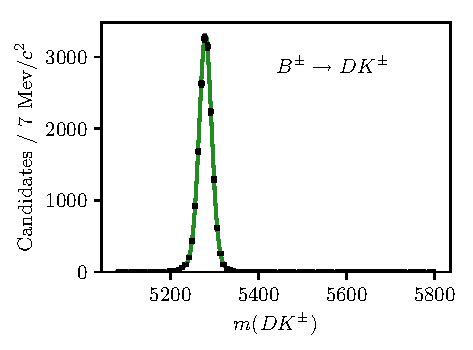
\includegraphics[width=0.45\columnwidth]{figures/analysis/pretty_mc_fit_signal_dk.pdf}
    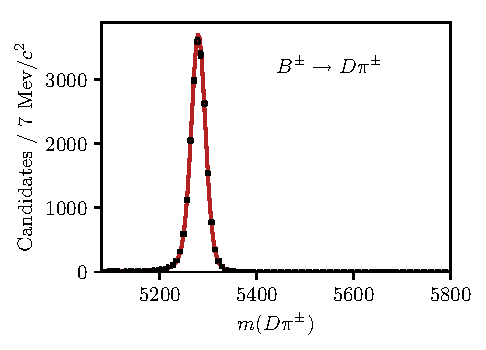
\includegraphics[width=0.45\columnwidth]{figures/analysis/pretty_mc_fit_signal_dpi.pdf}
    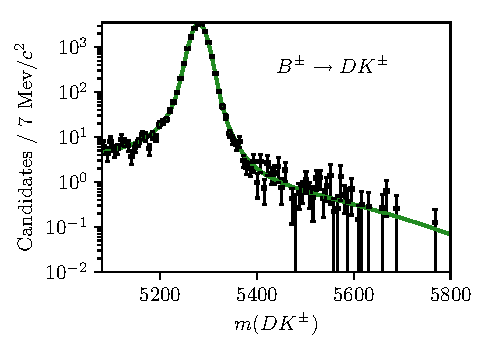
\includegraphics[width=0.45\columnwidth]{figures/analysis/pretty_mc_fit_signal_dk_log.pdf}
    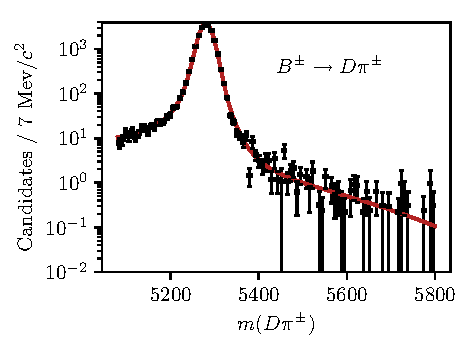
\includegraphics[width=0.45\columnwidth]{figures/analysis/pretty_mc_fit_signal_dpi_log.pdf}
    \caption{Fit projection of the signal shape to simulated $\Bpm\to\D(\to\KS\pip\pim)\hadron^\pm$ samples reconstructed in the LL category. (Left) shows \D\kaon shapes, and (right) shows $\D\pi$ shapes. The shapes are shown with both linear and logarithmic $y$-axis scales.}
    \label{fig:sig_shapes_mc}
\end{figure}


The signal component is modelled with a sum of a Gaussian density function, $f_G(m|m_B, \sigma)$, and a modified Gaussian distribution with the parameterisation
\begin{align}
    f_C(m|m_B, \sigma, \alpha_L, \alpha_R, \beta)\propto \left\{
    \begin{array}{ll}
    \exp\left[\frac{-\Delta m^2 (1+\beta \Delta m^2)}{2\sigma^2 + \alpha_L \Delta m^2}\right], & \Delta m = m - m_B  < 0 \\[8pt]
    \exp\left[\frac{-\Delta m^2 (1+\beta \Delta m^2)}{2\sigma^2 + \alpha_R \Delta m^2}\right], & \Delta m = m - m_B  > 0,
    \end{array} 
    \right.
\end{align}
which is Gaussian when $\Delta m^2 \ll \sigma^2/\alpha_{L/R}$ or $\Delta m^2 \gg \beta^{-1}$ (with widths of $\sigma$ and $\sqrt{\alpha_{L/R}/\beta}$ respectively), with an exponential-like transition that is able to model the effect of the experimental resolution of \lhcb very well. For the case $\beta=0$ the shape is denoted the \emph{Cruijff} shape; however, in this case it tends to a uniform distribution for large $\Delta m^2$ values, and cannot model the tails of the signal distribution. Thus, the full
density function is
\begin{align}
    f_s(m|m_B, \sigma, \alpha_L, \alpha_R, \beta) = k_C f_C(m|m_B, \sigma, \alpha_L, \alpha_R, \beta) + (1-k_C)f_G(m|m_B, \sigma).
\end{align}
The tail parameters $(\alpha_{L/R}, \beta)$ and the constant $k_C$ are determined in fits to simulated signal decays that have passed the full selection. The parameters are shared between the \Kspipi and \KsKK channels, but otherwise independent in the fit categories. An example of a fit to simulated $\Bpm\to\D(\to\Kspipi)h^\pm$ decays is given in Fig.~\ref{fig:sig_shapes_mc}. The resolution parameters $\sigma$ are determined in the fit to actual data. Separate parameters are determined in the LL and DD categories, because the LL category has a better resolution on the \Ks momentum, and therefore a narrow peak in reconstructed \B mass. Likewise, separate resolution parameters are used for \BtoDpi and \BtoDK decays, because the smaller $Q$ value in the latter case leads to smaller momenta of the decay products, and a correspondingly better resolution.



The signal yields are determined independently in each \BtoDpi category. The yields in the \BtoDK categories are then parameterised in terms of a single yield-ratio $\mathcal R_{K/\pi}$, and $\epsilon^c$, the corresponding selection efficiency for a given category
\begin{align}
    N^c_{\DK} = \mathcal R_{K/\pi} \times N^c_{\Dpi} \times \frac{\epsilon^c_{\DK}}{\epsilon^c_{\Dpi}}.
\end{align}
The selection efficiency is obtained in simulation, except for the PID efficiencies which are obtained in calibration data as described in Section~\ref{sub:particle_identification_requirements}. The parameter $\mathcal R_{K/\pi}$ is shared between all categories, and corresponds to the branching ratio between \BtoDK and \BtoDpi decays. Therefore, it can be compared to the known branching ratio~\cite{PDG2020}, which serves as an important cross check of the determination of relative efficiencies.




% subsection signal_decays (end)

\subsection{\texorpdfstring{Cross-feed between \BtoDh channels}{Cross-feed between BtoDh channels}} % (fold)
\label{sub:texorpdfstring_cross_feed_between_btodh_channels}

There is a cross-feed between the  $\BtoDpi$ and $\BtoDK$ channels, where real \BtoDpi decays are reconstructed as \BtoDK decays, or where \BtoDK decays are reconstructed as \BtoDpi decays. Due to relative branching fractions the former contribution is by far the most important, but both are modelled.


The cross-feed shapes are obtained in a data-driven manner using the sPlot method~\cite{sPlot}, and fixed in the fit to data. Separate shapes are determined for each category, using the following steps: 
\begin{figure}[tb]
    \centering
    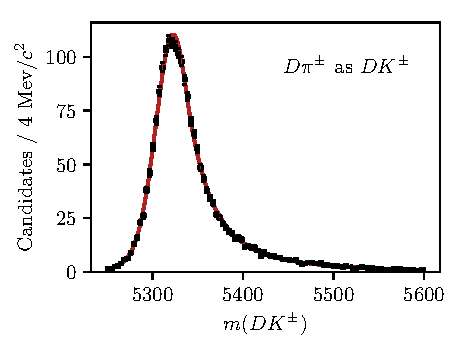
\includegraphics[width=0.45\columnwidth]{figures/analysis/pretty_sw_misID_dk_LL.pdf}
    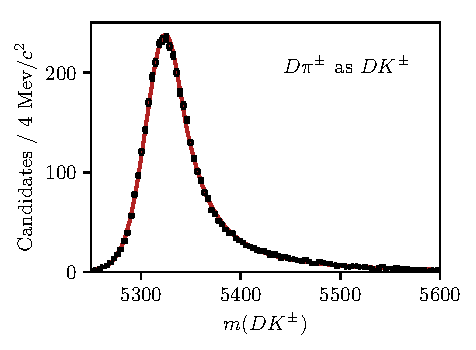
\includegraphics[width=0.45\columnwidth]{figures/analysis/pretty_sw_misID_dk_DD.pdf}
    \caption{Fitted shape of the \Bpm invariant mass spectrum for \BtoDpi decays misidentified as \BtoDK decays for (left) LL and (right) DD candidates in the \DtoKspp mode.}
    \label{fig:misid_shape_DPi_kspp}
\end{figure}

\begin{figure}[tb]
    \centering
    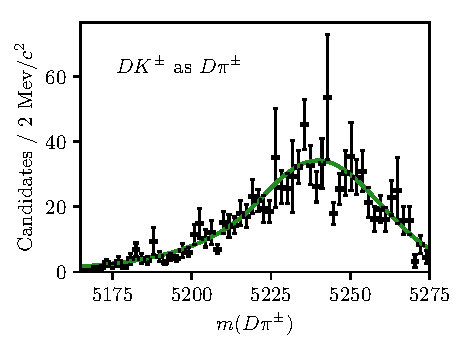
\includegraphics[width=0.45\columnwidth]{figures/analysis/pretty_sw_misID_dpi_LL.pdf}
    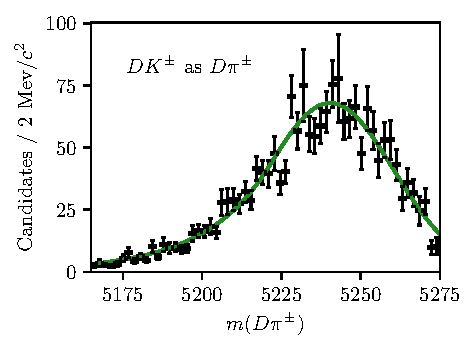
\includegraphics[width=0.45\columnwidth]{figures/analysis/pretty_sw_misID_dpi_DD.pdf}
    \caption{Fitted shape of the \Bpm invariant mass spectrum for \BtoDK decays misidentified as \BtoDpi decays for (left) LL and (right) DD candidates in the ${\DtoKspp}$ mode.}
    \label{fig:misid_shape_DK}
\end{figure}

\begin{itemize}
    \item The procedure is based on the reasonably pure \BtoDpi sample obtained when the full selection is applied. A simple mass fit is performed to the invariant mass spectrum and the sPlot method \cite{sPlot} is used to obtain the sWeights, $w_s$, for the signal component. The mass fit uses the same components for signal, low mass shape, and combinatorial background as described in this section. 

\item A set of weights are defined, based on the candidate-by-candidate PID efficiencies obtained as described in Section~\ref{sub:particle_identification_requirements}:
  \begin{itemize}
    \item The extracted PID efficiencies of the \texttt{PIDK}$<$4 cut $\epsilon_{\D\pi\to\D\pi}(p,\eta,n_\text{tracks})$ are used to reverse-weight the \BtoDpi sample, in order to obtain the bachelor kinematic distributions before the \texttt{PIDK}$<$4 cut is applied. 
    \item The extracted PID efficiencies of the \texttt{PIDK}$>$4 cut $\epsilon_{\D\pi\to\D\kaon}(p,\eta,n_\text{tracks})$ are used to obtain the bachelor kinematic distribution of the \BtoDpi candidates mis-identified as \BtoDK.
  \end{itemize}
  
\item The raw distribution of the invariant mass of \Bpm particles with  a misidentified bachelor, $m_B^{mis-ID}$, is produced by also doing the \texttt{DecayTreeFitter} kinematic refit while swapping the companion mass hypothesis of each \BtoDpi candidate to a kaon hypothesis.

\item Each candidate is reweighted by the overall weight $w=w_s^{cand.} / \epsilon_{\D\pi\to\D\pi}^{cand.} \cdot \epsilon_{\D\pi\to\D\kaon}^{cand.}$, and the reweighed $m_B^{mis-ID}$ distribution is fitted to obtain the cross-feed mass distribution function.
\end{itemize}
The distributions are modelled with a sum of two Crystal Ball density functions, each defined by the parameterisation~\cite{CrystalBall}
\begin{align}\label{eq:CB_definition}
  f_\text{CB}(m,\mu,\sigma,\alpha, n)\propto \left \lbrace
  \begin{array}{ll}
    \exp \left [ -\frac{1}{2}\left(\frac{m-\mu}{\sigma}\right)^2 \right] & \text{if   } (m-\mu)/\sigma > -\alpha  \\[8pt]
    A\left(B-\frac{m-\mu}{\sigma}\right)^{-n} & \text{otherwise,}\end{array}\right.
\end{align}
where $\alpha >0$, and
\begin{align}
  A &= \left(\frac{n}{\alpha}\right)^n\exp [-\alpha^2/2]\,, &
  B &= \frac{n}{\alpha}-\alpha\,.
\end{align}
The obtained $m_B^{mis-ID}$ spectrum and obtained mass shape is given in Fig.~\ref{fig:misid_shape_DPi_kspp} for the \DtoKspipi category; the \DtoKskk shapes are very similar. An analogous procedure is used to obtain the mass distribution of \BtoDK decays reconstructed in the \BtoDpi category. In the first stage where sPlots are extracted by a fit to the \BtoDK mass spectrum, the cross-feed component determined as described above is included. An example of one of the resulting shapes is given in Fig.~\ref{fig:misid_shape_DK}. The shape obtained in this manner performs better than one obtained using simulated decays, because the precision of the momentum determination is slightly overestimated in simulation.



The yield of cross-feed from \BtoDpi decays in a given \BtoDK category is parameterised in terms of the yield of correctly identified \BtoDpi decays and the mis-identification probability extracted from calibration samples as described in Section~\ref{sub:particle_identification_requirements}. Denoting the rate at which a pion is reconstructed as a kaon by $\epsilon_{\pi\to\kaon}^c$ in a given category, $c$, the yield is
\begin{align}
    N^c_{\pi\to\kaon} = N^c_{\Dpi} \frac{\epsilon_{\pi\to\kaon}^c}{1-\epsilon_{\pi\to\kaon}^c},
\end{align}
with an analoguous definition of the  yield of the cross-feed component from \BtoDK decays in the \BtoDpi spectrum. 


\subsection{Partially reconstructed backgrounds} % (fold)
\label{sub:partially_reconstructed_backgrounds}

A number of background candidates stem from partly reconstructed \B decays of the type $\B \to \D h X$, where $X$ denotes a photon or a pion that is not reconstructed.  It is not possible to reject these decays in the selection, due to the similarity to signal decays. The missing momentum results in reconstructed \B masses below the actual \B mass, and therefore the backgrounds are also denoted \emph{lowmass} backgrounds. These  mass distributions are modelled with analytic shapes, derived based on two principles.
Firstly, the kinematic endpoints of the distributions are fully defined by the particle masses in the decay. Secondly, the angular distribution of the missing particle has a one-to-one relation to the missing momentum, and therefore to the reconstructed $B$ mass.
Depending on the spin-parity of the particles and resonances involved in the decay, two different mass distributions arise. 

In \B decays where the missing particle is a scalar that is produced in the decay of a vector resonance (eg. $\Bpm\to\Dstarz(\to \Dz\piz) \pipm$ decays where the \piz is not reconstructed), the $m(\Dz\pipm)$ distribution has a double-peak structure. The \Dstarz helicity angle $\theta$ is defined as the angle between the \piz momentum vector in the \Dstarz rest frame and the \Dstarz boost vector in the $B$ rest frame. The helicity of the \Dstarz meson means that the \piz will travel predominantly in the direction where $\theta=0$ or $\theta=\pi$. When $\theta=0$ the fraction of momentum carried by the missing $\piz$ is lower, leading to a higher reconstructed $m(\Dz\pipm)$. When $\theta=\pi$ the converse occurs. The resulting \PB mass distribution is a parabola $f^0_\mathrm{HORNS}(m)$ peaking near both kinematic endpoints \Pa and \Pb
\begin{equation}
f^0_\mathrm{HORNS}(m) = \begin{cases}
 (m - \frac{a+b}{2})^2, & \text{if $a < m < b$} \\
  0, & \text{otherwise.}
\end{cases}
\end{equation}
Due to the double-peaking structure, and the fact that is was developed by Paolo Gandini for the two-body ADS/GLW analyses~\cite{LHCb-PAPER-2016-003}, this shape is denoted a \emph{HORNSdini} shape when convolved with a resolution function as described below.

The second relevant decay situation is where the missing particle is a vector, again produced via the intermediate decay of a vector resonance (eg. $\Bpm\to\Dstarz(\to \Dz\gamma) \pipm$ decays where the photon is not reconstructed).  In this case, the spin-parity of the phton ($1^-$) means that it will decay preferentially in the $\Ptheta = \frac{\pi}{2}$ or  $\Ptheta=\frac{3\pi}{2}$ directions, and so a double-peak structure is not seen. In this case the parabolic distribution $f^0_\mathrm{HILL}(m)$ with kinematic endpoints \Pa, \Pb has negative curvature and can be described by
\begin{equation}
f^0_\mathrm{HILL}(m) = \begin{cases}
-(m-a)(m-b), & \text{if $a < x < b$} \\
 0, & \text{otherwise.}
\end{cases}
\end{equation}
This shape is denoted a \emph{HILLdini} shape when convolved with a resolution function. A convolution is applied to take into the non-perfect resolution in the momentum determination. The resolution function is  chosen to be a sum of two Gaussians. For a single Gaussian shape $f_G(x|\mu,\sigma)$ with mean $\mu$ and width $\sigma$, the double Gaussian is expressed as
\begin{equation}\label{eq:pr_resolution}
f_{DG}(x) = f_G(x | \mu, \sigma) + k_G f_G(x|\mu,R_\sigma \sigma).
\end{equation}
where $\sigma$ is the width of the first Gaussian, $k_G$ is the relative fractions between the two Gaussians, and $R_\sigma$ is their relative widths.
Further, selection effects can distort the horns shape such that one of the peaks is higher than the other. This is taken into account by introducing a linear polynomial with slope parameter $\xi$. As $\xi\to 0$, the left hand peak decreases in size relative to the right hand peak.
The resulting \emph{HORNSdini} and \emph{HILLdini} distributions are therefore
\begin{equation}
f_\mathrm{HORNS/HILL}(m) = \int^b_a dx \; f^0_\mathrm{HORNS/HILL}(x) f_{DG}(m | x, \sigma, k_G, R_\sigma) \left( \frac{1-\xi}{b-a}x + \frac{b\xi-a}{b-a} \right).
\end{equation}
Examples of the shapes are given in Fig.~\ref{fig:HORNS_HILL_example}.  These shapes are used to fit all partially reconstructed backgrounds, as described in the following section.

\begin{figure}
\centering
\begin{subfigure}{0.49\columnwidth}
    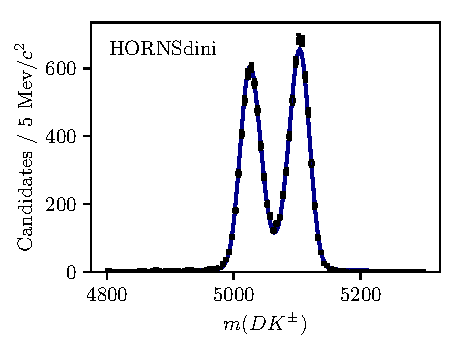
\includegraphics[width=\textwidth]{figures/analysis/pretty_HORNS.pdf}
    \caption{\label{fig:hornsdini}}
\end{subfigure}
\begin{subfigure}{0.49\columnwidth}
    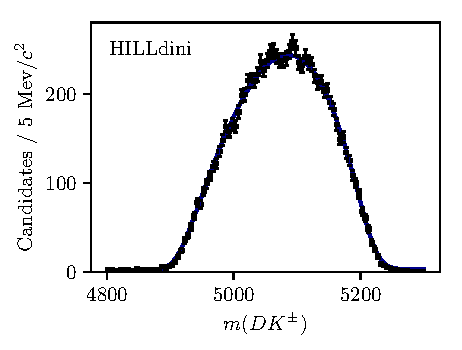
\includegraphics[width=\textwidth]{figures/analysis/pretty_HILL.pdf}
    \caption{\label{fig:hillsdini}}
\end{subfigure}
\caption{Examples of (a) the \emph{HORNSdini} distribution fit to simulated ${\Bpm\to(\Dstarz\to\Dz[\piz])\Kpm}$ decays, and
(b) the \emph{HILLSdini} distribution fit to simulated ${\Bpm\to(\Dstarz\to\Dz[\gamma])\Kpm}$ decays. The fits in this figure are made to illustrate the features of each shape, but do not enter the actual fit to data.
\label{fig:HORNS_HILL_example}}
\end{figure}

% Included background shapes
\subsubsection{Determination of the partially reconstructed background distributions}
In both the \BtoDK and \BtoDpi categories, components are included to describe contributions from the partially reconstructed decays
\begin{itemize}
\item $\Bpm\to(\Dstarz\to\Dz[\piz])h^\pm$, described using a \emph{HORNSdini} distribution,
\item $\Bpm\to(\Dstarz\to\Dz[\Pgamma])h^\pm$, described using a \emph{HILLdini} distribution
\item $\Bz\to(\Dstarpm\to\Dz[\pipm])h^\mp$, described using a \emph{HORNSdini} distribution,
\item $\B^{\pm(0)}\to \Dz h^\pm[\pi^{0(\mp)}]$, described using a \emph{HORNSdini} distribution,
\end{itemize}
where the particle in square brackets is not reconstructed. 
The mass distributions of all the $\B\to\Dstar h^\pm$ contributions are obtained from fits to samples of full \lhcb simulation. Examples of these fits are shown in Fig.~\ref{fig:sig_shapes_PR_dst}. All shape parameters are kept fixed in the fit to data, except for the parameter $\sigma$ of the resolution function in Eq.~\eqref{eq:pr_resolution} which is allowed to obtain the value preferred by data. 

\begin{figure}[tb]
    \centering
    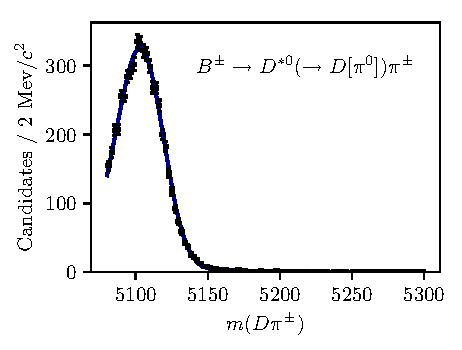
\includegraphics[width=0.45\columnwidth]{figures/analysis/pretty_mc_fit_low_dpi_Bu2Dst_pi0.pdf}
    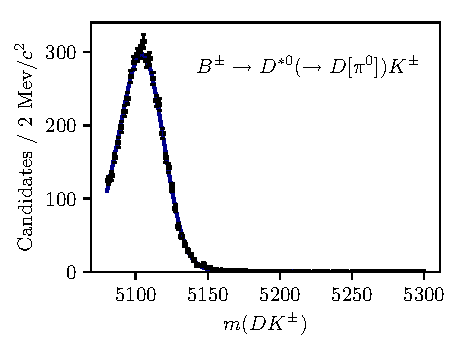
\includegraphics[width=0.45\columnwidth]{figures/analysis/pretty_mc_fit_low_dk_Bu2Dst_pi0.pdf}
    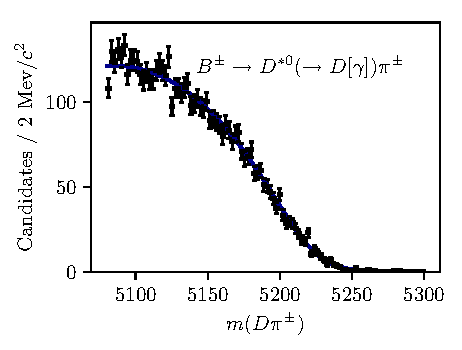
\includegraphics[width=0.45\columnwidth]{figures/analysis/pretty_mc_fit_low_dpi_Bu2Dst_gam.pdf}
    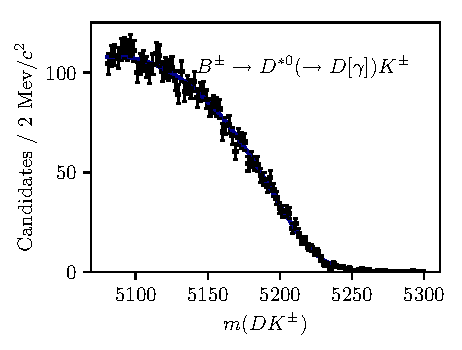
\includegraphics[width=0.45\columnwidth]{figures/analysis/pretty_mc_fit_low_dk_Bu2Dst_gam.pdf}
    \caption{Fit projection of the fit to (top) simulated ${\Bp\to\Dstarz(\to \Dz[\piz])h^\pm}$ decays and (bottom) simulated ${\Bp\to\Dstarz(\to \Dz[\gamma])h^\pm}$  decays, all reconstructed in the DD category. Both the (left) \D\kaon and (right) $\D\pi$ shapes are shown. }
    \label{fig:sig_shapes_PR_dst}
\end{figure}

\begin{figure}[tb]
    \centering
    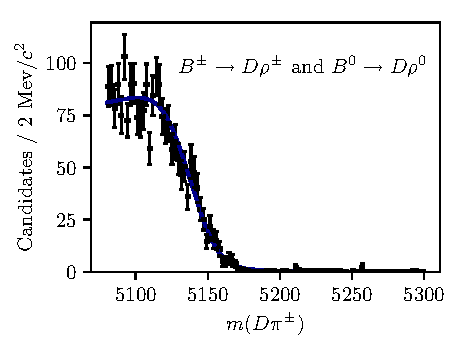
\includegraphics[width=0.45\columnwidth]{figures/analysis/pretty_mc_fit_low_dpi_B2Dpipi_LL.pdf}
    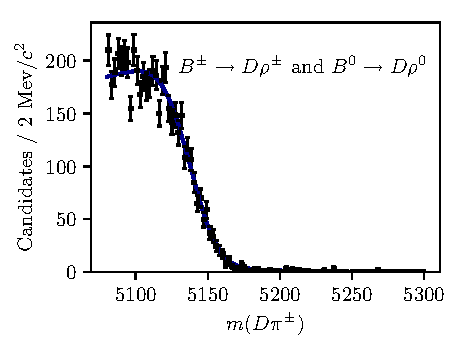
\includegraphics[width=0.45\columnwidth]{figures/analysis/pretty_mc_fit_low_dpi_B2Dpipi_DD.pdf}
    \caption{Projections of the fit to simulated $\Bpm\to\D\rhopm$ and $\Bz\to\D\rhoz$ samples reconstructed as $\Bpm\to\D\pipm$ decays for the (left) LL and (right) DD categories. }
    \label{fig:sig_shapes_PR_drho}
\end{figure}

The mass distribution of ${\B^{\pm}\to \Dz h^\pm[\pi^{0}]}$ and ${\B^{0}\to \Dz h^\pm[\pi^{\mp}]}$ decays reconstructed in the \BtoDpi categories is obtained from full \lhcb simulation samples of $\Bpm\to\Dz\rho^\pm$ and $\Bz\to\Dz\rho^0$ decays. The shapes were compared to those predicted by an amplitude model for $\B^{0}\to \Dz \pipm\pimp$ decays developed by \lhcb~\cite{LHCb-PAPER-2014-070}, but found to be very similar for the $m(\D \pipm)$ range relevant to this analysis. The obtained shapes are shown in Fig.~\ref{fig:sig_shapes_PR_drho}.

The mass distribution of ${\B^{\pm}\to \Dz \Kpm[\pi^{0}]}$ and ${\B^{0}\to \Dz \Kp[\pi^{-}]}$ decays reconstructed in the \BtoDK categories, on the other hand, is obtained from a sample of signal decays, generated via a an amplitude model for $\B^{0}\to \Dz \Kp\pim$ decays developed by \lhcb~\cite{LHCb-PAPER-2015-059} and smeared to take the \lhcb resolution into account. This follows an approach developed in the context of a GLW analysis based on partially reconstructed decays made within \lhcb~\cite{LHCb-PAPER-2017-021}. The obtained shape is shown in Fig.~\ref{fig:fit_part_reco_DKpi}.

\begin{figure}[tbp]
    \centering
    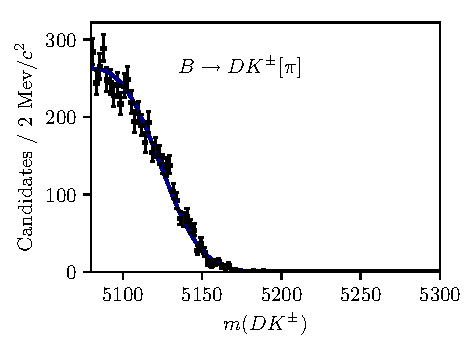
\includegraphics[width=0.45\textwidth]{figures/analysis/pretty_mc_fit_low_dk_B2DKpi.pdf}
    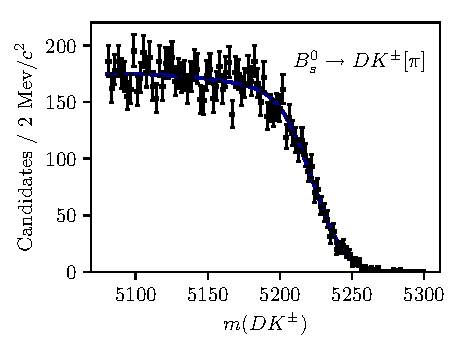
\includegraphics[width=0.45\textwidth]{figures/analysis/pretty_mc_fit_low_dk_Bs2DKpi.pdf}
    \caption{Fit projection for the fit used to obtain a shape for the partly reconstructed background from (left) $\B\to\D\kaon\pi$ decays and (right) $\Bs\to\D\Kp\pim$ decays where a pion is not reconstructed.}
    \label{fig:fit_part_reco_DKpi}
\end{figure}




% Yields
The background yields of these backgrounds are parameterised in terms of one total yield parameter, accounting for all partially reconstructed \Bpm and \Bz decays, and a number of parameters that describe the relative rates of the different contributions.
In the \BtoDpi channels, the relative rates of the $\Bpm\to(\Dstarz\to\Dz[\piz])h^\pm$ and $\Bz\to(\Dstarpm\to\Dz[\pipm])h^\mp$ backgrounds are fixed from the known branching fractions, and relative selection efficiencies in simulation. These backgrounds have almost identical mass distributions and it is not possible to determine the ratio in the fit to data. The relative yield of ${\Bpm\to\Dstar(\to \Dz[\gamma])\pi^\pm}$ compared to the $\B\to\Dstar(\to\Dz[\pi])\pi^\pm$ is denoted $f^{\D\pi}_{\Dstar\gamma}$ and is floated in the fit to data, as is the relative yield of $\B\to\Dz\pi^\pm[\pi]$ decays compared to the $\B\to\Dstar\pi$ modes, denoted $f^{\D\pi}_{\D\pi\pi}$. In the \BtoDK channels, all the relative background rates are fixed via known branching fractions and relative selection efficiencies; this is necessary to obtain a stable fit, due to the lower yields. 

% The Bs background
In the \BtoDK categories, an additional partially reconstructed background is considered from $\Bs\to\Dzb[\pi^+]\Km$ (and conjugate) decays. The mass shape is obtained from simulated decays, generated using an amplitude model published by \lhcb~\cite{LHCb-PAPER-2014-036} and smeared to account for the experimental resolution.  The obtained shape is shown in Fig.~\ref{fig:fit_part_reco_DKpi}. The yield of this background component is fixed relative to the signal yields in the corresponding \BtoDpi category, taking the relative efficiencies, branching ratios and hadronisation factors into account~\cite{PDG2020,LHCb-PAPER-2018-050}.



% Mis-ID components
In the \BtoDK channels there is a contribution from partially reconstructed $\B\to\Dstar\pipm X$ decays where the companion pion is misidentified as a kaon. The reverse contribution is negligible due to the relative branching fractions, and the fact that the $\kaon\to\pi$ misidentification shifts most of these background decays below the mass range of the fit. These are modelled using analytic, empirical mass distributions (essentially sums of a number of regular \emph{HORNS/HILLdini} distributions), with parameters  that are determined in fits to simulated $\B\to\Dstar\pipm$ and $\B\to\D\rho$ decays where the pion is reconstructed with the kaon mass hypothesis. The shapes are fixed in the fit to data.\\


% The non-included backgrounds
\subsubsection{Partially reconstructed backgrounds that are not modelled}
It was considered whether a background from $\Lb\to\Dz p\pim$ decays where a pion is not reconstructed,  and the proton is misidentified as the companion, can be expected to contribute significantly. This background has been investigated using full \lhcb simulation samples for the \D final state \KsPiPi. Taking into account the selection efficiencies, branching fractions, and hadronisation fraction of this background, the expected relative yield of the \Lb background compared to signal of 0.03\,\% in the \BtoDpi channel, which is completely negligible. In the \BtoDK channel the yield relative to signal is about 1.2\,\%, for total of about 200 decays. However, most of these lie at \B masses smaller than the signal peak, and their impact is small. Therefore it is not necessary to model the background in the nominal fit; a systematic uncertainty is assigned that accounts for the small potential impact. 

In the analogous case of $\Lb\to\Dz p\Km$ decays, the missing energy of the non-reconstructed kaon results in a reconstructed \B mass below the fit range.

It has also been investigated whether a background from $\Lb\to\Lc\pim$ or $\Lb\to\Lc\Km$ decays can be expected, where $\Lc\to p \KS \pip\pim$, a pion is missed and the proton is misidentified as a pion or kaon from the \D decay.  In practice, the background is sufficiently suppressed from the applied \D mass requirement to have no significant impact, and is therefore not modelled. A systematic uncertainty is assigned that accounts for any potential impact on the measurement due to this choice.



% subsection partially_reconstructed_backgrounds (end)

\subsection{Combinatorial background} % (fold)
\label{sub:combinatorial_background}

The combinatorial background is modelled with an exponentially falling density function, where both the yield and exponential slope are determined independently for each category. This shape is found to model the combinatorial well in all categories, most evident in the high-$m_B$ regions where this background dominates.





% subsection combinatorial_background (end)



% subsection texorpdfstring_cross_feed_between_btodh_channels (end)

\subsection{Fit results} % (fold)
\label{sub:global_fit_results}

\begin{figure}[tbp]
    \centering
    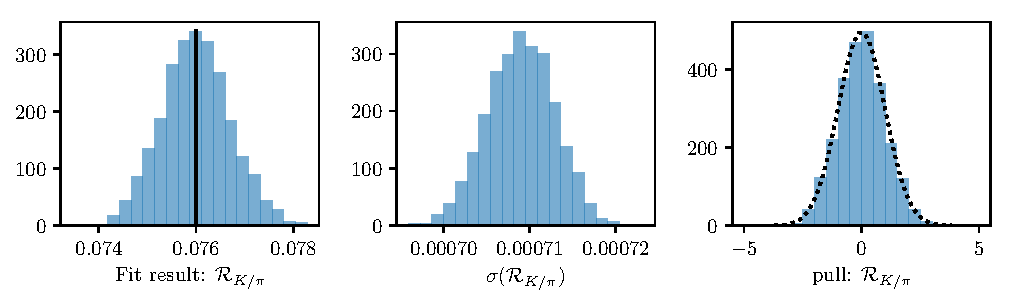
\includegraphics[width=0.85\columnwidth]{figures/analysis/pretty_feasibility_plots/pretty_feasibility_R.pdf}
    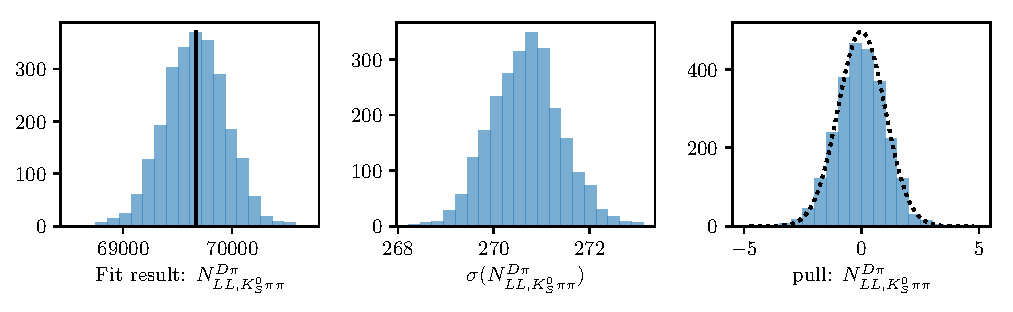
\includegraphics[width=0.85\columnwidth]{figures/analysis/pretty_feasibility_plots/pretty_feasibility_n_sig_dpi_d2kspp_LL.pdf}
    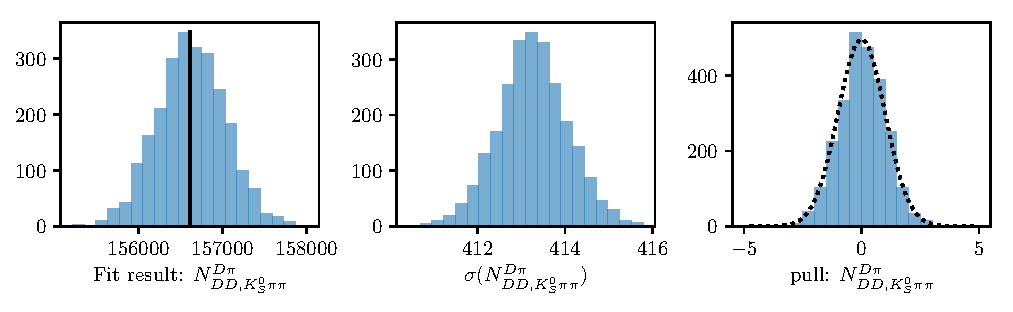
\includegraphics[width=0.85\columnwidth]{figures/analysis/pretty_feasibility_plots/pretty_feasibility_n_sig_dpi_d2kspp_DD.pdf}
    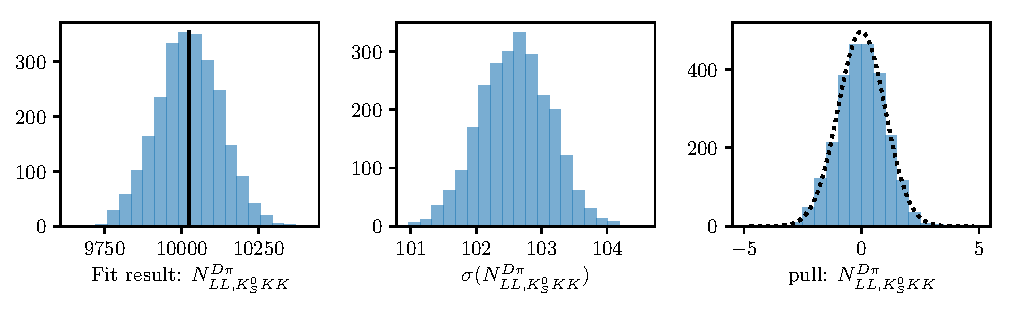
\includegraphics[width=0.85\columnwidth]{figures/analysis/pretty_feasibility_plots/pretty_feasibility_n_sig_dpi_d2kskk_LL.pdf}
    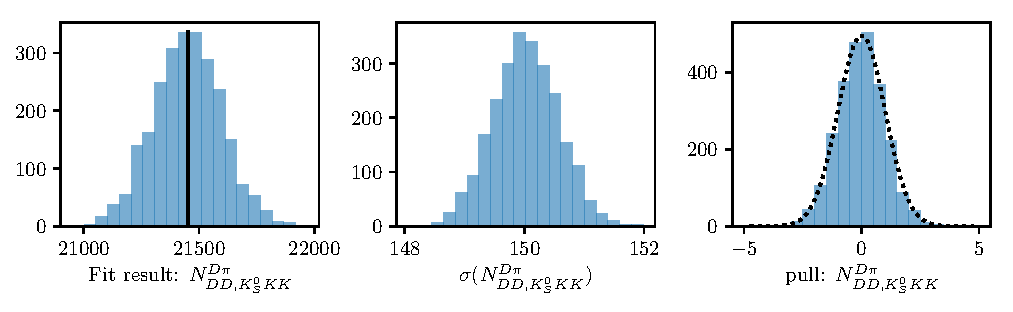
\includegraphics[width=0.85\columnwidth]{figures/analysis/pretty_feasibility_plots/pretty_feasibility_n_sig_dpi_d2kskk_DD.pdf}
    \caption{The (left) fitted value, (centre) estimated statistical uncertainty, and (right) pull plots for the signal yield parameters, as obtained in a number of pseudo experiments. The black line on the left shows the value used to generate the pseudo data sets; the dotted line on the right shows a Gaussian distribution with mean equal to zero and a standard deviation equal to unity.}
    \label{fig:global_fit_yield_pulls}
\end{figure}

The fit range is chosen to be $m_B\in[5080, 5800]\mevcc$. The low end of this interval includes the higher mass peak of the double-peak structure in the partially reconstructed background, which helps the fit constrain the relative contributions of backgrounds in the lowmass region. A number of additional backgrounds exist at even lower $m_B$ values, thus extending the fit range to lower masses would necessitates an extended model, but not benefit the description of the signal region. The high end of the interval includes enough combinatorial background to allow the fit to determine the exponential slope parameter accurately.


A large number of pseudoexperiments are carried out to verify that the fit procedure is self-consistent, in which toy data sets are generated according to the expected \B mass distributions, and then fitted. None of the parameters obtained in the fit exhibit a mean bias different from zero. For most parameters the uncertainties are well estimated.  This is the case for the signal yields, and the \DK--\Dpi yield ratio $\mathcal R_{K/\pi}$, as evidenced by the pull plots in Fig.~\ref{fig:global_fit_yield_pulls}. The fit underestimates the uncertainty by 10-20\,\% for some of the parameters related to the partly reconstructed backgrounds, as shown in Fig.~\ref{fig:lowmass_pulls}, but this is taken into account when the uncertainties are propagated to the observables in the second-stage fit, as described in Section~\ref{sub:systematics_from_mass_shapes}.



\begin{figure}[tbp]
    \centering
    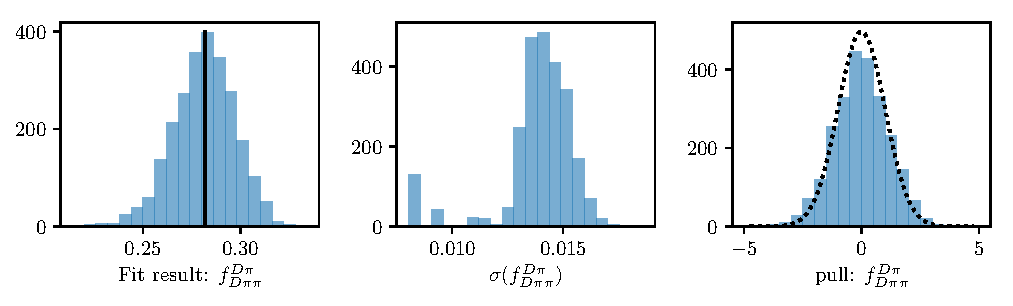
\includegraphics[width=0.85\columnwidth]{figures/analysis/pretty_feasibility_plots/pretty_feasibility_low_dpi_ratio_b2drho_vs_b2dstpi.pdf}
    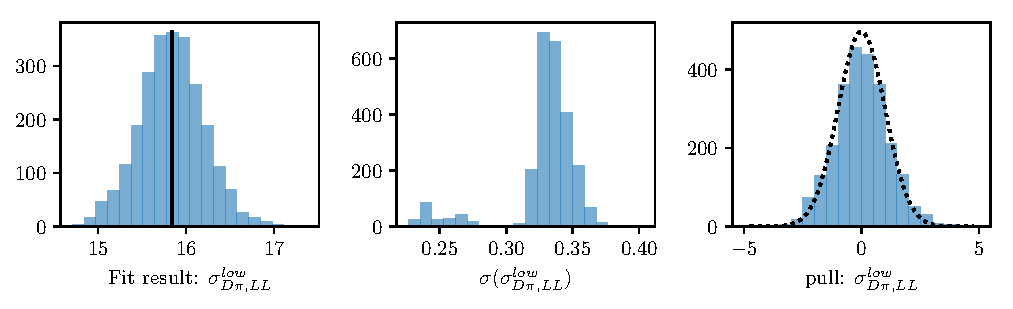
\includegraphics[width=0.85\columnwidth]{figures/analysis/pretty_feasibility_plots/pretty_feasibility_low_sigma_pi_LL.pdf}
    \caption{The (left) fitted value, (centre) estimated statistical uncertainty, and (right) pulls obtained in a number of pseudo experiments for two examples of parameters relating to the partially reconstructed backgrounds, where the uncertainties are slightly underestimated on average. The standard deviation of the pull distributions is approximately 1.15 in both cases.}
    \label{fig:lowmass_pulls}
\end{figure}


\begin{figure}[tp]
    \centering
    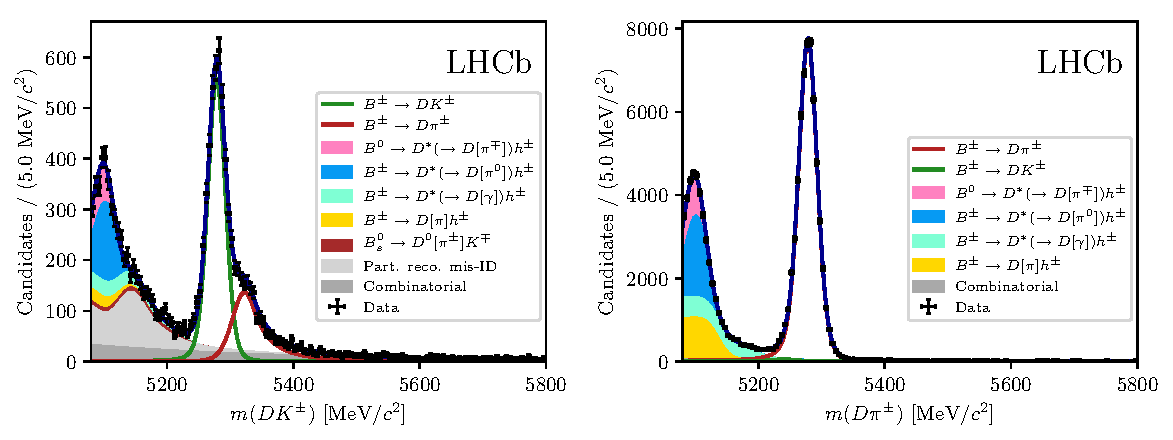
\includegraphics[width=0.98\columnwidth]{figures/analysis/pretty_fit_d2kspp_LL.pdf}
    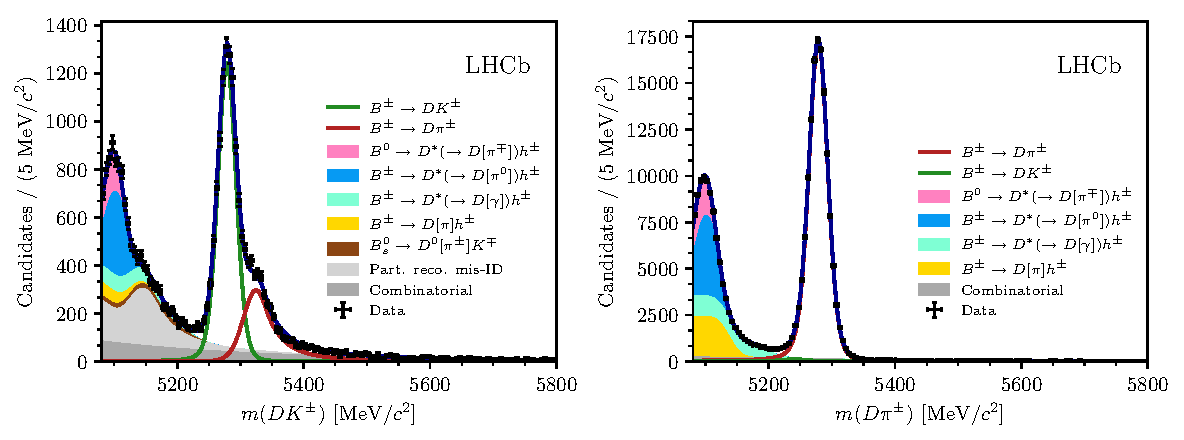
\includegraphics[width=0.98\columnwidth]{figures/analysis/pretty_fit_d2kspp_DD.pdf}
    \caption{The invariant mass distribution for the (left) \BtoDK channel and (right) \BtoDpi channel, where \DtoKspp and the \KS is in the (top) LL and (bottom) the DD categories. The particle within square brackets in the legend denotes the particle that has not been reconstructed. }
    \label{fig:kspipimass}
\end{figure}

\begin{figure}[tp]
    \centering
    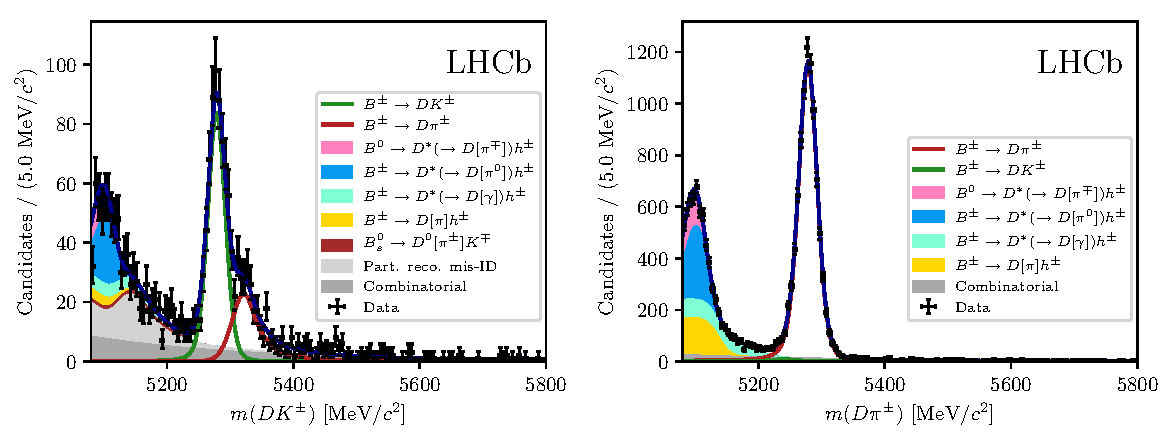
\includegraphics[width=0.98\columnwidth]{figures/analysis/pretty_fit_d2kskk_LL.pdf}
    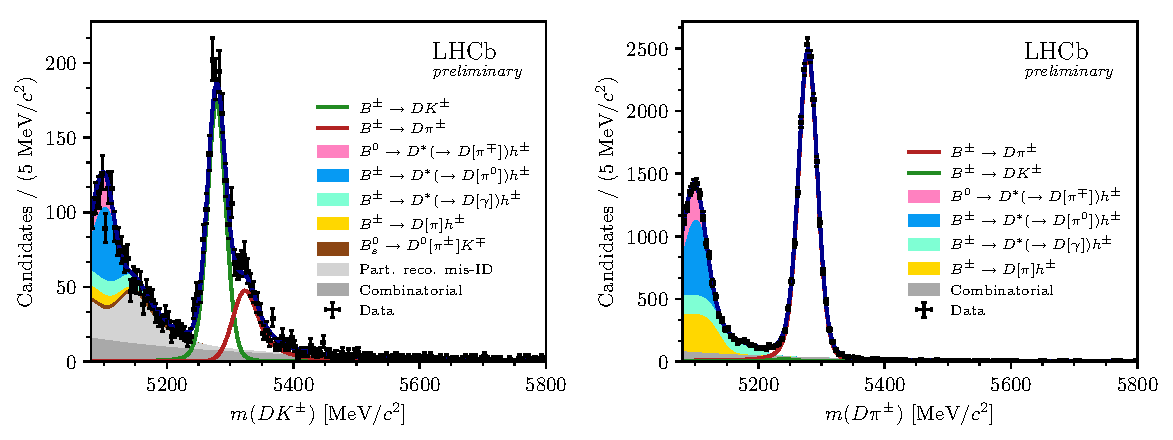
\includegraphics[width=0.98\columnwidth]{figures/analysis/pretty_fit_d2kskk_DD.pdf}
    \caption{The invariant mass distribution for the (left) \BtoDK channel and (right) \BtoDpi channel, where \DtoKskk and the \KS is in the (top) LL and (bottom) the DD categories. The particle within square brackets in the legend denotes the particle that has not been reconstructed.}
    \label{fig:kskkmass}
\end{figure}

The projections of the fit to data are shown in Figs.~\ref{fig:kspipimass}~and~\ref{fig:kskkmass}, for the ${\DtoKspipi}$ and \DtoKsKK data sets, respectively. The obtained yields for each fit component are given in Table~\ref{tab:yields_global_fit}. The total yield of \BtoDpi decays is approximately 230,000 across all channels. The obtained value of the yield ratio is $\mathcal R_{K/\pi}=(7.7\pm0.1)\,\%$, corresponding to a total \BtoDK yield of 16,500, of which about 14,300 pass the PID requirement and are reconstructed in the \BtoDK category. This value of $\mathcal R$ is in excellent agreement with expectation from the known branching fractions~\cite{PDG2020}, which predict $\mathcal R_{K/\pi}^\text{PDG}=(7.8\pm0.3)\,\%$.\footnote{While it would seem this measurement thus determines the yield ratio $\mathcal R_{K/\pi}$ with a much better precision than the current world average uncertainty, that is because the result quoted here does not include any systematic uncertainties; it is only included to serve as a, successfully passed, cross check.} The shape parameters determined in the fit to data are summarised in Table~\ref{tab:fitted_parameters_global_fit}.

% text autogenerated via ANA_scripts/05_cp_fit/RunFitAndExtractResults.ipynb
\begin{table}[tp]
\centering
\renewcommand{\arraystretch}{1.2}
\caption{Fitted total candidate yields. 
The quoted signal yields are for the number of candidates that survive the respective PID cut, whereas the \DK-\Dpi ratio is corrected for PID and selection efficiencies so that it corresponds to the branching ratio.
\label{tab:yields_global_fit}
}
\begin{tabular}{l c c}

\toprule
Component& LL & DD \\ 
\midrule\multicolumn{3}{c}{Signal} \\
\midrule 
\BtoDpiDtoKspp     & $61,573\pm254$      &   $139,080\pm389$                 \\
\BtoDpiDtoKskk     & $9,160\pm98$        & $19,910\pm144$          \\
\cline{2-3}
$R_{\kaon/\pi}=n(DK)/n(D\pi)$ (\%)        & \multicolumn{2}{c}{$7.72\pm0.08$}               \\
\midrule 
\multicolumn{3}{c}{Combinatorial} \\
 \midrule 
\BtoDpiDtoKspp     & $3,479\pm198$ & $9,928\pm376$ \\
\BtoDpiDtoKskk     & $1,103\pm94$ & $2,545\pm155$ \\
\BtoDKDtoKspp      & $1,826\pm107$  & $3,987\pm177$  \\
\BtoDKDtoKskk      & $380\pm39$  & $655\pm58$  \\
\midrule 
\multicolumn{3}{c}{Part. Reco.} \\
 \midrule 
\BtoDpiDtoKspp     & $43,004\pm242$      &   $95,452\pm403$                 \\
\BtoDpiDtoKskk     & $6,247\pm99$        & $13,241\pm157$          \\
\cline{2-3}
$R_{\kaon/\pi}^{low}=n_{low}(DK)/n_{low}(D\pi)$ (\%)        & \multicolumn{2}{c}{$6.65\pm0.12$}             \\
\bottomrule
\end{tabular}
\renewcommand{\arraystretch}{1.0}
\end{table}
 
% text autogenerated via ANA_scripts/05_cp_fit/RunFitAndExtractResults.ipynb
\begin{table}[tb]
\renewcommand{\arraystretch}{1.2}
\centering
\caption{Fitted parameter values. \label{tab:fitted_parameters_global_fit}}
\begin{tabular}{l c c}
\toprule
& LL & DD \\
\midrule
$\sigma_{D\pi}$ (MeV/$c^2$)             & $14.27\pm0.05$    & $14.58\pm0.04$ \\
$\sigma_{DK}$ (MeV/$c^2$)               & $13.61\pm0.24$     & $14.19\pm0.17$ \\
\cline{2-3}
$\mu$ (MeV/$c^2$)                       & \multicolumn{2}{c}{$5278.60\pm0.04$} \\
\midrule 
\multicolumn{3}{c}{Combinatorial Slopes} \\
Decay mode & \multicolumn{2}{c}{Slope $(10\times 10 ^{-3}GeV^{-1} c^2$)} \\ 
 \midrule
\BtoDpiDtoKspp                         & $-3.1\pm0.2$ & $-4.0\pm0.1$ \\
\BtoDpiDtoKskk                         & $-4.1\pm0.4$ & $-5.5\pm0.3$ \\
\BtoDKDtoKspp                          & $-3.2\pm0.2$  & $-3.9\pm0.2$ \\
\BtoDKDtoKskk                          & $-4.2\pm0.4$  & $-4.3\pm0.4$ \\
\midrule 
\multicolumn{3}{c}{Part. Reco.} \\
 \midrule
$\sigma_{D\pi}^{low}$ (MeV/$c^2$)      & $13.73\pm0.33$    & $13.78\pm0.28$ \\
\cline{2-3}
$f_{\D\pi\pi}^{\D\pi} $                 & \multicolumn{2}{c}{$0.268\pm0.013$} \\
$f_{\Dstar\gamma}^{\D\pi} $             & \multicolumn{2}{c}{$0.317\pm0.005$} \\
\bottomrule
\end{tabular}
\renewcommand{\arraystretch}{1.0}
\end{table}

% subsection fit_results (end)

% section signal_and_background_components (end)
\FloatBarrier
\section{Measurement of the CP-violation observables} % (fold)
\label{sec:measurement_of_the_cp_violation_observables}

The section describes the second fit stage, in which the \CP-violation observables of interest are determined. Compared to the first fit stage, the candidates are further split by \B charge, and by the assigned Dalitz bin number, making for a total of 160 subcategories.\footnote{In the thesis, the word \emph{category} is used for the 8-way split of data by companion species, \KS track type, and \D-decay mode, indexed with a $c$; the word \emph{bin} denotes the 16 (4) regions of the \DtoKspp (\DtoKskk) Dalitz plots, indexed with an $i$; the simultaneous grouping by \emph{category}, \emph{bin}, and \B charge is denoted a \emph{subcategory}, of which there are $4\times 2 \times (16+4)=160$.} Another extended maximum-likelihood fit is carried out, in which shape parameters of all signal and background components are fixed to those determined in the first fit stage, and all floating parameters relate to the signal and background yields. The signal yields are expressed in terms of the observables of interest, $(\xpmdk, \ypmdk, \xxidpi, \yxidpi)$, allowing the fit to determine their optimal values. The details of the fit setup are summarised in the following section, along with a number of studies that lead to the specific setup being chosen. The results are presented in Section~\ref{sub:main_cpfit_results}, and a wide range of consistency checks are described in Section~\ref{sub:cpfit_cross_checks}.

\subsection{Fit setup} % (fold)
\label{sub:fit_setup}

The basic principle of the measurement is that the signal yields in each bin (in a given category) are defined using the equations of Chapter~\ref{ch:2-litreview}, in order to allow for the determination of the \CP-violation observables. In practice, a set of variables are defined
\begin{align}\label{eq:Y_definition}
    Y^-_{c,i} &= F_{c,\phantom{-}i} + [(\xm^c)^2 + (\ym^c)^2] F_{c,-i} + 2\sqrt{F_{c,i}F_{c,-i}}\left(\ci^c\xm^c+\si^c\ym^c\right), \\
    Y^+_{c,i} &= F_{c,-i} + [(\xp^c)^2 + (\yp^c)^2] F_{c,\phantom{-}i} + 2\sqrt{F_{c,i}F_{c,-i}}\left(\ci^c\xp^c-\si^c\yp^c\right),
\end{align}
for each data category, $c$, in terms of which the bin yields that enter the likelihood are given by
\begin{align}
    N^\pm_{c, i} = \frac{Y^\pm_{c, i}}{\sum_j Y^\pm_{c,j}}\times N^\pm_{c,\text{ total}}.
\end{align}
This parameterisation is essentially identical to the expressions in Section~\ref{sec:strategy_for_lhcb_measurement}, slightly modified so that the phase-space-integrated yields of \Bp and \Bm decays in a given category are determined directly, in lieu of the normalisation constants $h^\pm$ of that section. As discussed briefly in Section~\ref{sec:strategy_for_lhcb_measurement}, there are choices to be made in terms of how the $x$ and $y$ are parameterised in the \BtoDpi channel, and how the \Fi parameters are determined. A series of feasibility studies were carried out to determine the optimal setup; these are presented in the following section, before the final fit setup is described in detail.

\subsubsection{Feasibility of alternative fit setups} % (fold)
\label{ssub:feasibility_of_alternative_fit_setups}

% subsubsection feasibility_of_alternative_fit_setups (end)

% 3) 
% i) why do you need to use 6 parameters rather than 8 (you mash up the DK and Dpi CPV parts so there needs to be a good motivation to have done this)
% ii) what is the expected contribution to the gamma uncertainty from 230K(or similar) B->Dpi events in this simultaneous fit (signal only) assuming a certain value for rBDpi
% iii) what would the precision on gamma be if the Fi were known perfectly. 
% I think you have all these studies done, so just a case of writing it up. 

% I think this is important as a) you refer to a paper that i think hints that the parameterisation of the xi variables gains statistical precision and you don’t want that idea percolating. b) more importantly this is a new method and so some of the basic studies of the method should be presented, and in particular the behaviour with different values of rBDpi and the impact that you get from running the fit in a certain way. 
% For example, if we had found that using the Dpi sample to get Fi added about 2 degrees to the uncertainty then we might have considered going back to the drawing board and trying to fix/correct the MC. 
% This is very much a key part of your intellectual contribution to the development of this analysis - i think it a real shame to omit this. In total i don’t think this would be more than a page or two depending on whether you thought plots were required or not but it is an essential piece of the work you have done. 

The motivation for promoting the \BtoDpi channel to a signal channel is two-fold: one aim is to extract the information on $\gamma$ from the \BtoDpi data, even the precision gain is limited, and another is to be able to the \Fi parameters directly from the \BtoDh channels, to avoid the need for a control channel and a simulation-reliant efficiency correction. Two different sets of observables can be defined to describe the \CP-violation effects in the \BtoDpi channel:
\begin{itemize}
    \item one option, defined the 8-parameters setup below,  is to define a new set of four Cartesian for the \BtoDpi mode, $(\xmdpi, \ymdpi, \xpdpi, \ypdpi)$, defined analogously to the \BtoDK observables
    \begin{align}
        \xpmdpi &= \rB^{D\pi} \cos (\dB^{D\pi} \pm \g), & \ypmdpi &= \rB^{D\pi} \sin (\dB^{D\pi} \pm \g),
    \end{align}
    \item another, proposed in Refs.~\cite{Tico:2018qmg,JordiXi2}, is to introduce the parameter
    \begin{subequations}
    \begin{align}
        \xi_{\DPi} = \left(\frac{r_B^{\DPi}}{r_B^{\DK}}\right)\exp [i (\delta_B^{\DPi}-\delta_B^{\DK})]
    \end{align}
    and then determine the observables
    \begin{align}
        \xxidpi &= \Re [\xi_{\Dpi}] & \yxidpi &= \Im [\xi_{\Dpi}].
    \end{align}
    \end{subequations}
    This is denoted the 6-parameters setup below. In terms of \xxidpi and \yxidpi, the usual Cartesian \xpm and \ypm are given by
    \begin{align}\label{eq:xy_from_xi}
        x_\pm^{\D\pi} &= x_\xi^{\D\pi}x_\pm^{DK} - y_\xi^{\D\pi}y_\pm^{DK}, 
        & y_\pm^{\D\pi} &= x_\xi^{\D\pi}y_\pm^{DK} + y_\xi^{\D\pi}x_\pm^{DK}.
    \end{align} 
\end{itemize}
The former parameterisation has the benefit that information on $\gamma$ from the \BtoDK and \BtoDpi channels is encoded in separate sets of observables, whereas the latter parameterisation encodes information on \CP violation from both channel in the $(\xpmdk, \ypmdk)$ parameters. In combinations of many measurements, it is a useful cross check to be able to compare constraints obtained from individual decay modes; a good example is the \lhcb combination from 2016~\cite{LHCb-PAPER-2016-032} where both \BtoDK and \BtoDh combinations are made and compared in detail. This is only possible with the former parameterisation. On the other hand, the latter parameterisation avoids the introduction of two non-physical degrees of freedom, which, as seen below, leads to better statistical behaviour.

In order to inform the choice of parameterisation, a series of pseudo experiments has been carried out to compare the obtainable precision on $\gamma$ (these studies were performed, and discussed within \lhcb, prior to the publication of Ref.~\cite{JordiXi2}; thus, the results presented here constitute independent work, even if there is some overlap in scope and conclusions with that reference). Many simulated data sets were generated, constituting of a number signal yields approximately equal to the expected yields in the full Run~1~and~2 \lhcb data set: approximately 15,000 \BtoDK decays and 210,000 \BtoDpi decays.\footnote{No backgrounds were included in these studies, and thus the quoted uncertainties on $\gamma$ are better than what is obtainable in the final measurement; a similar study including realistic backgrounds is presented for the final setup below.} The signal decays were distributed between Dalitz bins according to  $(\gamma, r_B^{DK}, \delta_B^{DK})=(75^\circ, 0.1, 130^\circ)$ in the \BtoDK mode, which is to the world average values of direct $\gamma$ measurements at the time. In the \BtoDpi mode, the behaviour is investigated for different sets of input values; of most importance is the case $(r_B^{D\pi}, \delta_B^{D\pi})=(0.005, 300^\circ)$, because it corresponds to the solution in the \lhcb combination~\cite{LHCb-PAPER-2016-032} that is in agreement with the theoretical expectation $r_B^{D\pi}\simeq 0.005$~\cite{rDpi}. The behaviour at larger $r_B^{D\pi}$ values is also investigated.
%, exemplified below by the parameter set $(r_B^{D\pi}, \delta_B^{D\pi})=(0.03, 330^\circ)$ which corresponds to the alternative solution in the \lhcb combination. 
For each generated data set
\begin{enumerate}
     \item the observables are measured in a fit to the data set, using both the 6-parameter and 8-parameter setups
     \item the obtained observables are then fitted to obtain the underlying physics parameters $(\gamma,r_B^{DK}, \delta_B^{DK}, r_B^{D\pi}, \delta_B^{D\pi})$ using a maximum-likelihood fit, essentially following the procedure outlined in Section~\ref{sub:statistical_approach}.
 \end{enumerate} 
 In the 8-parameter setup it is possible to determine $\gamma$ using the results in either the \BtoDK or \BtoDpi channels separately, or consider the combined results; in the 6-parameter setup only the latter option is available. The studies are performed in two modes: with the \Fi floating in the fit, emulating a realistic fit to data, as well as with the \Fi fixed to the input values used in data generation. The latter studies emulate a setup where the \Fi parameters are determined in an ultra-high statistics control channel, and perfect efficiency corrections are applied. In all cases, a single set of \Fi parameters is shared between the \BtoDK and \BtoDpi modes.

\begin{figure}[tb]
    \centering
    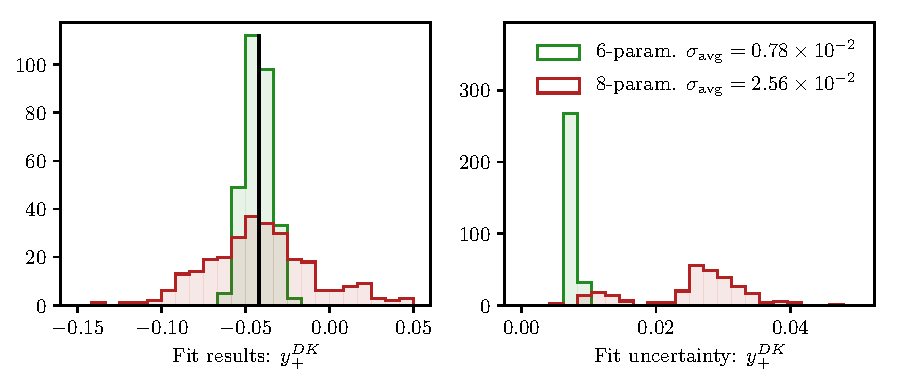
\includegraphics[width=0.95\columnwidth]{figures/analysis/signal_only_feasibility_thesis/compare_68_yp.pdf}
    \caption{The distribution of (left) fit values and (right) statistical uncertainty estimate for \ypdk in a series of pseudo experiments, for both the (green) 6-parameter and (red) 8-parameter setups.}
    \label{fig:compare_yp_68}
\end{figure}

The 6-parameter setup shows significantly better statistical performance than the 8-parameter setup in the realistic case where the \Fi parameters are determined in the fit and $r_B^{D\pi}\sim 0.005$.\footnote{For larger, non-physical values of $r_B^{D\pi} > 0.03$ both fit setups behave well.} The fits that employ the 6-parameter setup behave well in this case, whereas the additional degrees of freedom in the 8-parameter fit leads to essentially all parameters being 100\,\% (anti-)correlated, and a significant number of fits not converging. For the fits that do converge, the uncertainties on the observables are significantly larger due to the large correlations, as shown exemplified with the case of $\ypdk$ in Fig.~\ref{fig:compare_yp_68}. This essentially determines the choice of parameterisation: it is possible to reliably model \CP violation in the \BtoDpi channel and simultaneously determine the \Fi parameters by using the 6-parameter setup, but not by using the 8-parameter setup.



Interestingly, when the constraints on $\gamma$ are compared, both setup lead to similar precision; in spite of the large uncertainties on the individual observables in the 8-parameter setups, the constraints on $\gamma$ are tight. This is illustrated in Fig.~\ref{fig:compare_g_68}. Nevertheless, it remains true that the 8-parameter setup is ruled out due the statistical behaviour in the determination of the observables.

\begin{figure}[tb]
    \centering
    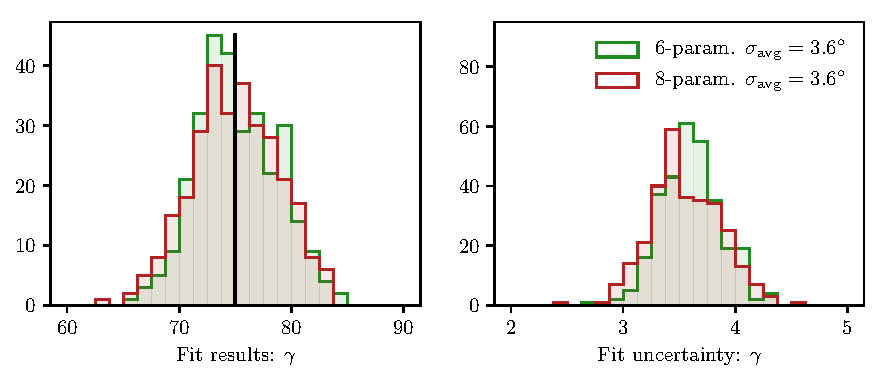
\includegraphics[width=0.95\columnwidth]{figures/analysis/signal_only_feasibility_thesis/compare_68_g.pdf}
    \caption{The distribution of (left) fit values and (right) statistical uncertainty estimate for $\gamma$ in a series of pseudo experiments, for both the (green) 6-parameter and (red) 8-parameter setups.}
    \label{fig:compare_g_68}
\end{figure}

Furthermore, both the 6- and 8-parameter setups lead to fits that behave well in the studies where the \Fi parameters are kept fixed, and the resulting uncertainties on the Cartesian observables and $\gamma$ are essentially identical. Thus, the 6-parameter setup does not inherently lead to a gain in precision over the 8-parameter setup; the strength of the parameterisation is that it allows for a reliable, simultaneous determination of the \Fi parameters and the observables of interest. This conclusion differs somewhat from the one drawn in Ref.~\cite{JordiXi2}.

The fixed-\Fi studies allow for an assessment of the gain in precision on $\gamma$ due to the inclusion of the \BtoDpi mode, by comparing the precision obtained in the simultaneous fits with that obtained when $\gamma$ is constrained using only information from the \BtoDK channel. In the realistic case where $r_B^{D\pi}=0.005$, the gain in precision is about $0.1^\circ$.
The reason for the small impact, in spite of the yield being approximately 14 times larger in the \BtoDpi channel than in the \BtoDK channel, is that $r_B$ is 20 times smaller, and the \CP asymmetries are proportional to $r_B$. Thus, the main improvement to the analysis from including \BtoDpi as a signal channel comes from the ability to determine the \Fi parameters without adding a large systematic uncertainty.\footnote{If this comparison is made using the parameter set $(r_B^{D\pi}, \delta_B^{D\pi})=(0.03, 330^\circ)$, which corresponds to the alternative, non-physical solution in the \lhcb combination~\cite{LHCb-PAPER-2016-032}, the gain in precision from the \BtoDpi channel is $1.3^\circ$ in stead, resulting in a final uncertainty of about $2.3^\circ$. This fact made the statistical interpretation of the \BtoDh combination in Ref.~\cite{LHCb-PAPER-2016-032} non-trivial.}



Finally, it is worth considering whether any precision can be gained by including further information on the \Fi parameters from a control channel, even if the fit is well behaved without external information. The potential yield in the ${\Bzb\to\Dstarp(\to \Dz \pip)\mu^- \bar \nu_\mu X}$ control channel is approximately three times larger than in the \BtoDpi channel, and it does therefore offer a better statistical handle on the \Fi values (at the significant cost of having to worry about efficiency corrections). This question can be answered by comparing the obtained precision on $\gamma$ in the fits where \Fi parameters were floating, to the precision in the case where they were kept fixed. Such a comparison is shown for the 6-parameter setup in Fig.~\ref{fig:compare_g_float_fixed} for the realistic scenario where $r_B^{D\pi}=0.005$. The difference in the average $\sigma(\gamma)$ is \emph{less than $0.05^\circ$}, which is of course completely negligible. Therefore, no gain in precision can be obtained by including the control channel in the analysis, and it is not considered further.
%\footnote{In the alternative case, where $r_B^{D\pi}=0.03$, the \BtoDpi mode drives the precision on $\gamma$, and YYY. However, the analysis design is chosen mainly based on the $r_B^{D\pi}=0.005$ case that is close to the theory expectation, and in any case, this gain in statistical precision would be compromised by the necessary efficiency correction, and the associated systematic uncertainty.}

\begin{figure}[tb]
    \centering
    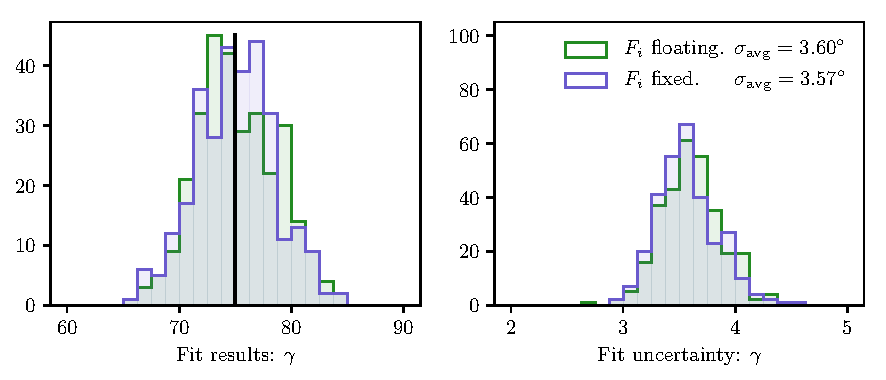
\includegraphics[width=0.95\columnwidth]{figures/analysis/signal_only_feasibility_thesis/compare_float_fix_g.pdf}
    \caption{The distribution of (left) central values and (right) statistical uncertainty estimate for $\gamma$ in a series of pseudo experiments that use the 6-parameter setup, where (green) the \Fi parameters are determined in the fit and (blue) where they are kept fixed at their input values.}
    \label{fig:compare_g_float_fixed}
\end{figure}

\subsubsection{Final choice of observables and the determination of the \texorpdfstring{\Fi}{Fi} parameters} % (fold)
\label{ssub:final_choice_of_observables}

% subsubsection final_choice_of_observables (end)

In the chosen setup, a single set of four parameters, $(\xmdk, \ymdk, \xpdk, \ypdk)$, are shared between \emph{all} \BtoDK categories; they enter the expressions of Eq.~\eqref{eq:Y_definition} directly, and are thus determined in the fit. In the \BtoDpi categories, the four corresponding parameters, $(\xmdpi, \ymdpi, \xpdpi, \ypdpi)$, are parameterised in terms of $(\xpmdk, \ypmdk)$ and the additional two observables $(\xxidpi, \yxidpi)$. The \Fi parameters are determined in the fit, being shared between the \BtoDK and \BtoDpi channels. However, separate parameter sets are determined for the LL and DD categories because the acceptance profile over the Dalitz plot differs between them. 



% subsubsection reparameterisation_of_the_texorpdfstring (end)
The \Fi parameters are subject to the constraint that $\sum_{i=-\mathcal N}^{\mathcal N} F^c_i=1$, for each category, $c$. Therefore, it is beneficial to introduce a reparameterisation in the likelihood function, where the \Fi parameters are expressed in terms of a set of recursive fractions
\begin{align}\label{eq:Ri_definition}
     \mathcal R_i = \left\{
     \begin{array}{ll}
         F_i  &,\quad i = -\mathcal N \\
         F_i \left/\left(\sum_{j\geq i}F_j\right)\right. &,\quad -\mathcal N < i < +\mathcal N \\
     \end{array}
     \right.,
 \end{align}
for which the constraint is much simpler, namely that each individual $\mathcal R_i$ parameter lies in the interval $[0, 1]$. This parameterisation leads to well behaved fits, where the $\mathcal R_i$ parameters do not suffer from significant correlations.

\subsubsection{Strong-phase inputs} % (fold)
\label{ssub:strong_phase_inputs}

The strong-phase parameters $(\ci, \si)$ are fixed in the fit to data. In the \DtoKspipi channels, the combined CLEO~\cite{CLEOCISI} and BESIII~\cite{BESCISI} measurement results are used, as reported in Ref.~\cite{BESCISI}. The \DtoKsKK categories also use combined CLEO~\cite{BESCISI} and BESIII results~\cite{BESCISIKSKK}, which are reported in Ref.~\cite{BESCISIKSKK}. The experimental uncertainty on these measurements is propagated to the measured \CP-violation observables as part of the systematic uncertainties in Section~\ref{sub:strong_phase_uncertainties}.


% subsubsection strong_phase_inputs (end)

\subsubsection{Treatment of backgrounds} % (fold)
\label{ssub:treatment_of_backgrounds}

% subsubsection treatment_of_backgrounds (end)
The yield of combinatorial background decays is determined independently in each bin. A single, overall bin yield of partially reconstructed background from \Bpm and \Bz decays is determined in each of the 160 subcategories; the relative contribution from each individual background is fixed from the results of the first-stage fit, corrected for the different fit region (a systematic uncertainty is assigned due to this choice). In the \BtoDK channels, the bin yields of the partially reconstructed background from $\Bs\to\Dzb[\pi^+]\Km$ decays are expressed via the \Fi, exploiting that a positive companion particle is always produced along with a \Dzb meson (and vice versa). The overall yield is fixed from the results of the first stage fit. Finally, the yield of the $\Dpi\leftrightarrow\DK$ cross-feed components in each bin are determined via the obtained yield of correctly identified decays in the corresponding bin, and the known PID efficiencies. This is true for both fully and partially reconstructed decays, although only a $\Dpi\to\DK$ component is included in the latter case. 

\subsubsection{The choice of fit range} % (fold)
\label{ssub:the_choice_of_fit_range}

% subsubsection the_choice_of_fit_range (end)

The fit range is decreased to $m_B\in[5150, 5800]\mevcc$. The information from candidates with lower reconstructed \B masses was useful in determining the relative rates and free mass shape parameters of the partially reconstructed background components in the first-stage fit; however, with these fixed in the second-stage fit, this is no longer the case. Furthermore, the setup assumes that the shape of the partially reconstructed background is identical across the Dalitz bins. This assumption is not perfectly true, but the impact is minimal when the lower limit of the fit range is taken to be 5150\mevcc, as described further in Section~\ref{ssub:using_the_same_part_reco_shape_in_all_dalitz_bins_ignoring_physics_effects_in_the_lowmass_background}.

\subsubsection{Self-consistency check} % (fold)
\label{ssub:self_consistency_check}

In order to establish the fit stability and investigate a potential bias, a series of pseudo experiments are run, in which data sets are generated using the model, and then fitted back. The total yields are taken from the first-stage fit. The signal yields are distributed between Dalitz bins using input physics parameters that approximately equal the values obtained in Section~\ref{sub:main_cpfit_results} from the results of the fit to data. The \Fi parameters are taken from a fit to data. The partly reconstructed background is distributed as "\Dz-like", ie. in the \Bpm channels $N_i^\pm\propto F_{\mp i}$, except for the \Bs background, which is "\Dzb-like" ($N_i^\pm\propto F_{\pm i}$).
The combinatorial background includes real \D mesons paired with a random bachelor, as well as fake \D mesons that are themselves made up of random tracks. The former is distributed as 50/50 \Dz-like and \Dzb-like in the toy generation, whereas the latter is assumed to be evenly distributed over the Dalitz plot (ie. the bin yield is proportional to the bin area).


\begin{table}
    \centering
    \caption{Mean biases and pulls for the observables of interest in the final, binned fit, obtained in a large number of pseudo experiments.
    \label{tab:cp_fit_toy_pulls}
    }

%autogenerated by 05_cp_fit/SensitivityAndBiasStudies.ipynb
\renewcommand{\arraystretch}{1.1}
\begin{tabular}{c|ccc}
\toprule
Parameter  & Mean bias $(\times 10 ^ {-2})$ & Mean pull & Pull width \\
\midrule
$\xmdk$                        & $            -0.018 \pm 0.022$& $-0.01\pm0.02$& $1.01\pm0.02$\\
$\ymdk$                        & $            -0.014 \pm 0.026$& $-0.00\pm0.02$& $0.99\pm0.02$\\
$\xpdk$                        & $            -0.018 \pm 0.022$& $-0.01\pm0.02$& $1.00\pm0.02$\\
$\ypdk$                        & $            -0.016 \pm 0.028$& $0.01\pm0.02$& $1.00\pm0.02$\\
$\xxidpi$                      & $\phantom{-}0.029 \pm 0.052$& $0.06\pm0.02$& $1.00\pm0.02$\\
$\yxidpi$                      & $\phantom{-}0.000 \pm 0.060$& $0.01\pm0.02$& $1.00\pm0.02$\\
\bottomrule
\end{tabular}
\renewcommand{\arraystretch}{1.0}

\end{table}

\begin{figure}[tp]
    \centering
    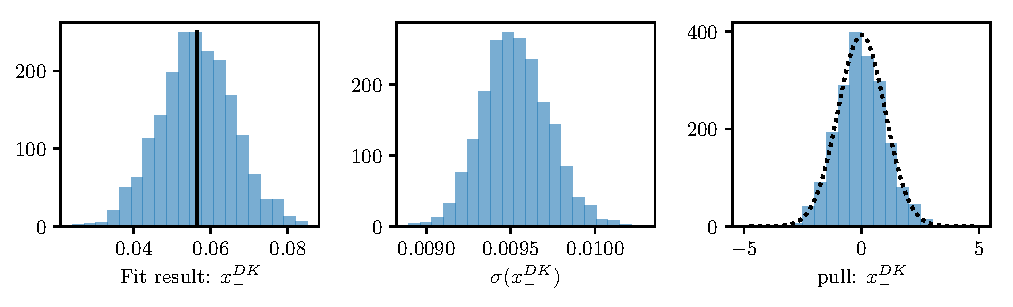
\includegraphics[width=0.85\columnwidth]{figures/analysis/pretty_feasibility_plots/pretty_feasibility_xm_dk.pdf}
    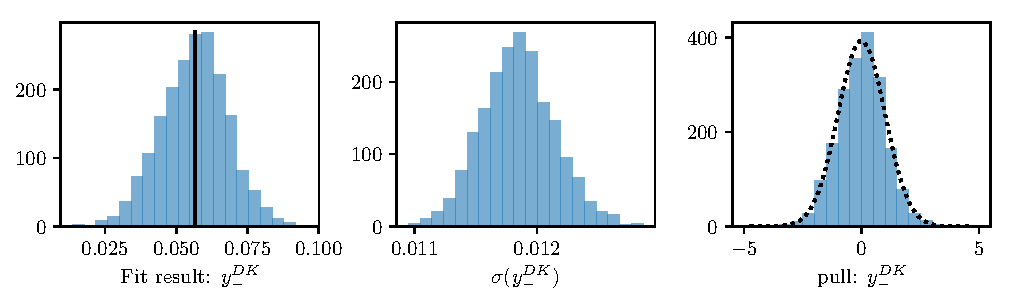
\includegraphics[width=0.85\columnwidth]{figures/analysis/pretty_feasibility_plots/pretty_feasibility_ym_dk.pdf}
    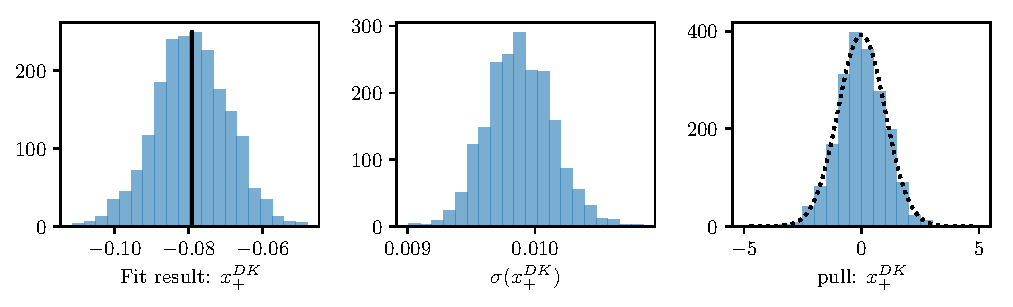
\includegraphics[width=0.85\columnwidth]{figures/analysis/pretty_feasibility_plots/pretty_feasibility_xp_dk.pdf}
    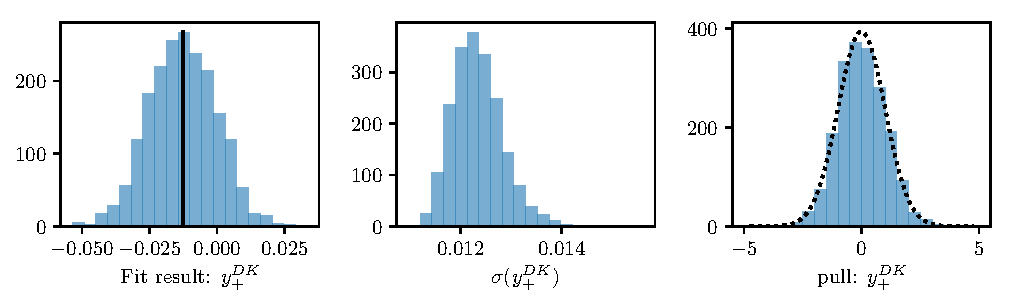
\includegraphics[width=0.85\columnwidth]{figures/analysis/pretty_feasibility_plots/pretty_feasibility_yp_dk.pdf}
    \caption{The (left) fitted value, (centre) estimated statistical uncertainty, and (right) pulls for the \BtoDK observables, as obtained in a number of pseudo experiments. The black line on the left shows the value used to generate the pseudo data sets; the dotted line on the right shows a Gaussian distribution with mean equal to zero and a standard deviation equal to unity.}
    \label{fig:cp_fit_pull_plots}
\end{figure}

\begin{figure}[tp]
    \centering
    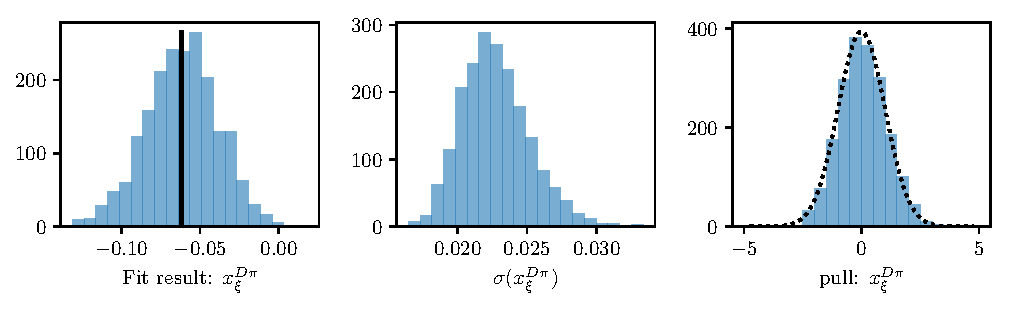
\includegraphics[width=0.85\columnwidth]{figures/analysis/pretty_feasibility_plots/pretty_feasibility_Re_xi_dpi.pdf}
    \includegraphics[width=0.85\columnwidth]{figures/analysis/pretty_feasibility_plots/pretty_feasibility_Im_Xi_dpi.pdf}
    \caption{The (left) fitted value, (centre) estimated statistical uncertainty, and (right) pulls for the \BtoDpi observables, as obtained in a number of pseudo experiments. The black line on the left shows the value used to generate the pseudo data sets; the dotted line on the right shows a Gaussian distribution with mean equal to zero and a standard deviation equal to unity.}
    \label{fig:cp_fit_pull_plots_dpi}
\end{figure}

% text autogenerated by ANA_scripts/05_cp_fit/SensitivityAndBiasStudies.ipynb
% biases from toy: 20200127_feasibility_study_model_cisi_take2
A set of 2000 pseudo experiments has been run, out of which 98.8\,\% converged properly. The pull plots for the observables of interest are shown in Figs.~\ref{fig:cp_fit_pull_plots}~and~\ref{fig:cp_fit_pull_plots_dpi}; the mean biases and pulls are summarised in Table~\ref{tab:cp_fit_toy_pulls}. No biases are statistically significant, and the uncertainties are seen to be well estimated. 

% subsubsection self_consistency_check (end)
% subsection fit_setup (end)

\subsection{Main results} % (fold)
\label{sub:main_cpfit_results}
% 
% \input{tables/cp_fit/cp_fit_results}

The values and statistical uncertainties of observables obtained in the fit are 
\begin{align}\label{eq:xy_fit_results}
% \begin{split}
    \xmdk   &= (\phantom{-}5.68\pm0.96)\times 10^{-2}, & \notag
    \ymdk   &= (\phantom{-}6.55\pm1.14)\times 10^{-2}, \\
    \xpdk   &= (         - 9.30\pm0.98)\times 10^{-2}, &
    \ypdk   &= (         - 1.25\pm1.23)\times 10^{-2}, \\
    \xxidpi &= (         - 5.47\pm1.99)\times 10^{-2}, & \notag
    \yxidpi &= (\phantom{-}0.71\pm2.33)\times 10^{-2}.
% \end{split}
\end{align}
The statistical correlation matrix for the observables is given in Table~\ref{tab:stat_corr_matrix}. None of the correlations are larger than 15\,\% and the values of both uncertainties and correlation coefficients are similar to those obtained in the feasibility studies. The 2D log-likelihood profile for the observables is shown in Fig.~\ref{fig:loglikelihood}, based on a full likelihood scan, where the fit is repeated with the observables fixed to a range of values around the optimal solution. It can be seen in the figure that the likelihood profile obtained in the scan is very well modelled by the Gaussian approximation, based on the Hessian matrix at maximum likelihood. Thus, the statistical uncertainties quoted in Eq.~\eqref{eq:xy_fit_results} are likely to be accurate.
The signature of \CP violation is that $(\xpdk, \ypdk) \neq (\xmdk, \ymdk)$, very clearly the case for the measurement results. Finally, the figure illustrates how the opening angle between the two points defined by $(\xpdk, \ypdk)$ and $(\xmdk, \ymdk)$ is equal to $2\gamma$.

\begin{figure}[t]
    \centering
    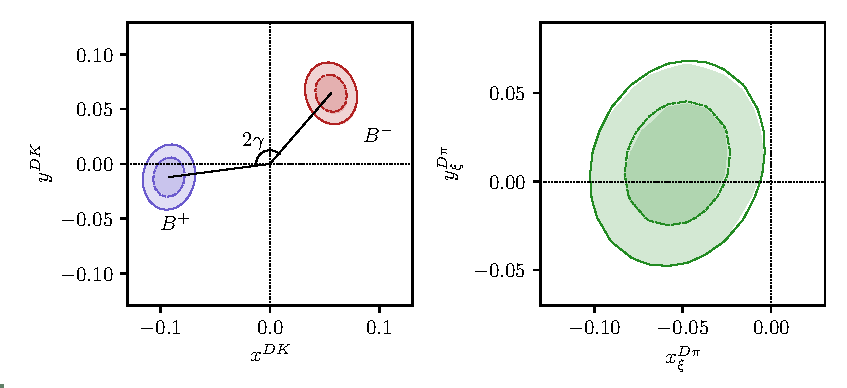
\includegraphics[width=0.9\columnwidth]{figures/analysis/likelihood_plot.pdf}
    \caption{The 68\,\% and 95\,\% confidence regions for the fitted observables. The lines show the regions estimated from the covariance matrix returned by the default fit. The shaded areas are obtained in a likelihood scan, where the binned fit is run many times with all observables held at fixed values, scanning pairs of observables over the relevant ranges. The scan is made separately for the three pairs $(\xmdk,\ymdk)$, $(\xpdk, \ypdk)$, and $(\xxidpi, \yxidpi)$, holding the four other parameters fixed at their default-fit central values during a given scan. Then the minimum log-likelihood is related to a $\chi^2$ via $\mathcal L_\text{min} = \frac{1}{2}\chi^2$ (discarding an irrelevant constant), and the confidence region limits placed at $\chi^2=2.30$ and $\chi^2=6.18$, yielding the relevant percentiles for a $\chi^2$ distribution with 2 degrees of freedom.}
    \label{fig:loglikelihood}
\end{figure}

The full set of fit projections in all 160 subcategories is included in Appendix~\ref{app:main_fit}. 
While the \CP asymmetry of the phase-space integrated yield is small, this is not the case for all individual bin-pairs. This is shown in Fig.~\ref{fig:kspipimass_bin2} where, as an example, the fit projections for the $\Bp\to\D\Kp$ decays in bin $+2$ and the $\Bm\to\D\Km$ decays in bin $-2$ of the \DtoKspipi Dalitz plot are compared. The presence of \CP violation is clearly visible.

\begin{figure}[t]
    \centering
    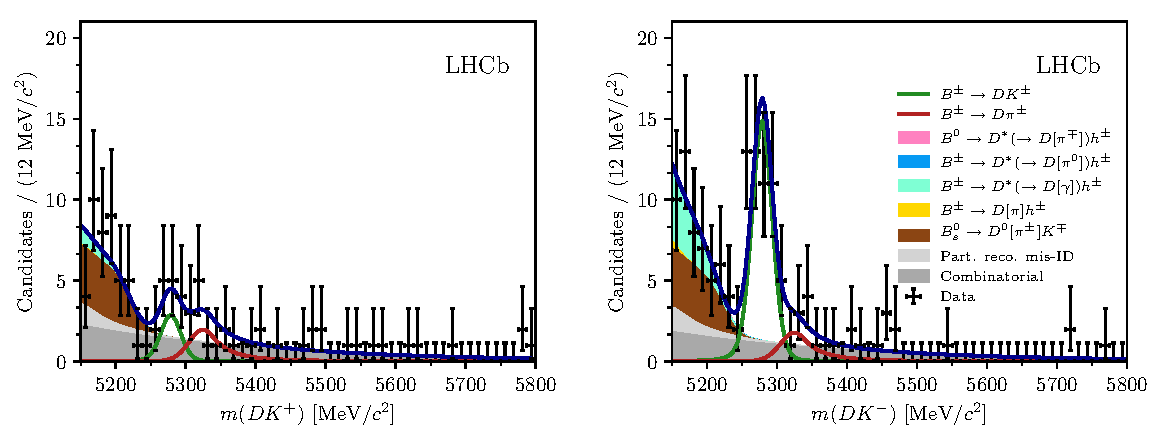
\includegraphics[width=0.9\columnwidth]{figures/analysis/pretty_fit_bin2_asym_comparison.pdf}
    \caption{The invariant mass distribution for the (left) $\Bp\to\D\Kp$ candidates in bin -2 and (right) the $\Bm\to\D\Km$ candidates in bin +2, where \DtoKspipi and the \KS is reconstructed in the DD category. }
    \label{fig:kspipimass_bin2}
\end{figure}

\begin{table}[tbp]
\centering
\caption{Statistical uncertainties and correlation matrix for the fit to data. 
\label{tab:stat_corr_matrix}}

% autogenerated via ANA_scripts/05_cp_fit/RunFitAndExtractResults.ipynb
\begin{tabular}{l|cccccc}
\toprule
\multicolumn{7}{c}{Uncertainty $(\times 10^{-2})$}\\ \midrule
 & $x_-^{\DK}$ & $y_-^{\DK}$ & $x_+^{\DK}$ &$ y_+^{\DK}$ & $x_\xi^{\Dpi}$ &$ y_\xi^{\Dpi} $\\
\midrule
$\sigma$ & $0.96$ & $1.14$ & $0.96$ & $1.20$ & $1.99$ & $2.34$ \\
\bottomrule \multicolumn{7}{c}{} \\
\multicolumn{7}{c}{Correlations}\\ \midrule
 &$ x_-^{\DK}$ & $y_-^{\DK}$ & $x_+^{\DK}$ &$ y_+^{\DK}$ & $x_\xi^{\Dpi}$ &$ y_\xi^{\Dpi} $\\
\midrule
$x_-^{\DK} $    & $\phantom{-}1.000$ & $-0.125$ & $-0.013$ & $\phantom{-}0.019$ & $\phantom{-}0.028$ & $-0.165$ \\
$y_-^{\DK} $    &    & $\phantom{-}1.000$ & $-0.011$ & $-0.009$ & $\phantom{-}0.105$ & $\phantom{-}0.030$ \\
$x_+^{\DK} $    & &       & $\phantom{-}1.000$ & $\phantom{-}0.088$ & $-0.099$ & $\phantom{-}0.038$ \\
$y_+^{\DK} $    & & &          & $\phantom{-}1.000$ & $-0.076$ & $-0.141$ \\
$x_\xi^{\Dpi}$ & & &     &         & $\phantom{-}1.000$ & $\phantom{-}0.146$ \\
$y_\xi^{\Dpi}$ & & &     &    &         & $\phantom{-}1.000$ \\
\bottomrule
\end{tabular} 


\end{table}



The obtained \Fi parameter values are shown in Table~\ref{tab:Fi_values}. These parameters can be useful in other BPGGSZ measurements made within the \lhcb collaboration: it is expected that the systematic uncertainty due to differences between the Dalitz-plot acceptance profile in \BtoDh decays and, say, $\B\to\Dstar\kaon$ or $\B\to\D\Kstar$ decays is smaller than the systematic arising from extracting the efficiency profile from simulated decays. Therefore, the obtain central values and uncertainties have been made public~\cite{GGSZ-B2Dh}, including a set of systematic uncertainties discussed in Section~\ref{sub:summary_of_systematic_uncertainties}.\footnote{In practice, it is the obtained $\mathcal R_i$ values that are made public, related to the \Fi parameters via Eq.~\eqref{eq:Ri_definition}.}




% printed via ANA_scripts/06_systematics/Fi_Systematics.ipynb
% reordered manually
\begin{table}
\centering

\caption{The fitted $\Fi$ values including statistical uncertainties. The underlying $\mathcal R_i$ values are given with both statistical and systematic uncertainties in Section~\ref{ssub:output_needed_for_other_ggsz_analyses}.
\label{tab:Fi_values}
}

\begin{tabular}{lcc}
\toprule
\multicolumn{3}{c}{$\Fi$ values: $\DtoKspipi$}\\
\midrule
bin &                 LL &                 DD \\
\midrule
-8  &  $0.024 \pm 0.001$ &  $0.024 \pm 0.000$ \\
-7  &  $0.127 \pm 0.001$ &  $0.133 \pm 0.001$ \\
-6  &  $0.062 \pm 0.001$ &  $0.056 \pm 0.001$ \\
-5  &  $0.046 \pm 0.001$ &  $0.042 \pm 0.001$ \\
-4  &  $0.095 \pm 0.001$ &  $0.095 \pm 0.001$ \\
-3  &  $0.160 \pm 0.001$ &  $0.160 \pm 0.001$ \\
-2  &  $0.153 \pm 0.001$ &  $0.153 \pm 0.001$ \\
-1  &  $0.095 \pm 0.001$ &  $0.097 \pm 0.001$ \\
 1  &  $0.022 \pm 0.001$ &  $0.020 \pm 0.000$ \\
 2  &  $0.005 \pm 0.000$ &  $0.005 \pm 0.000$ \\
 3  &  $0.004 \pm 0.000$ &  $0.004 \pm 0.000$ \\
 4  &  $0.055 \pm 0.001$ &  $0.056 \pm 0.001$ \\
 5  &  $0.027 \pm 0.001$ &  $0.022 \pm 0.000$ \\
 6  &  $0.004 \pm 0.000$ &  $0.003 \pm 0.000$ \\
 7  &  $0.055 \pm 0.001$ &  $0.057 \pm 0.001$ \\
 8  &  $0.067 \pm 0.001$ &  $0.072 \pm 0.001$ \\
\midrule \\

\multicolumn{3}{c}{$\Fi$ values: $\DtoKsKK$}\\

\midrule
bin &                 LL &                 DD \\
\midrule
-2  &  $0.207 \pm 0.004$ &  $0.202 \pm 0.003$ \\
-1  &  $0.222 \pm 0.004$ &  $0.230 \pm 0.003$ \\
 1  &  $0.290 \pm 0.005$ &  $0.296 \pm 0.003$ \\
 2  &  $0.281 \pm 0.005$ &  $0.271 \pm 0.003$ \\
\bottomrule
\end{tabular}
\end{table}


% subsection main_results (end)

\subsection{Cross checks} % (fold)
\label{sub:cpfit_cross_checks}


A series of cross checks are performed to verify that the fit to data is behaving as expected.

\subsubsection{Comparison to results of earlier analyses} % (fold)
\label{ssub:comparison_to_results_of_earlier_analyses}

It is confirmed that the results obtained in fits of the Run~1 or 2015+16 data sets in isolation are compatible with the results obtained in the original \lhcb analyses of those data sets~\cite{LHCb-PAPER-2014-041,LHCb-PAPER-2018-017}. In order to do so, the whole analysis procedure is carried out using only the relevant subset of data, and the strong-phase inputs from the CLEO collaboration are used in the fit. Two effects need to be taken into account when comparing the central values.

Firstly, the overlap between the data samples is not 100\,\% due to changes in the candidate selection. The overlap between the new selection and the data set of the original analysis  of Run~1 data is about 70\,\%, whereas is it about 90\,\% for the 2015+16 data set. In order to determine the expected difference between the observables fitted from data sets with significant overlap, a large number of toy data sets were generated in sets of two, where 70 (90)\,\% of decays were shared between the data sets. Both data sets were fitted and the difference between the obtained central values for each observable tabulated; the standard deviation of these distributions are used to calculate the pulls between the old analysis results and the new fits to data. This check does not take into account that the semi-leptonic PID cuts were introduced to remove a potential peaking background, which may have had a small systematic effect on the earlier measurement results. Thus the expected differences are likely to be slightly underestimated and the check is conservative.

Furthermore, the $F_i$ parameters were determined in a semi-leptonic control channel in the earlier analyses. Therefore, the expected difference obtained above is adjusted by adding the $F_i$-related systematic uncertainty of the original analysis in quadrature, when comparing the old results to those in new fits to the Run~1 and 15+16 data sets. No further corrections have been made to the expected differences, which effectively assumes all other systematic uncertainties to be 100\,\% correlated. Also for this reason can the check be considered conservative. As can be seen in Tables~\ref{tab:comparison_run1_results}~and~\ref{tab:comparison_1516_results}, neither the Run~1 and 2015+16 comparisons show unreasonable differences in central values.

\begin{table}
\centering
\caption{
    Comparison between the results on the Run~1 analysis~\cite{LHCb-PAPER-2014-041} and the central values obtained when fitting the Run~1 dataset with the selection and fit setup described in this note. The pull is calculated using the $1\sigma$ expected difference, which takes the sample overlap and the systematic uncertainty on the $F_i$ parameters in the previous analysis into account, but assumes all other systematic uncertainties to be perfectly correlated. The new fits are performed using the CLEO strong-phase inputs.
    \label{tab:comparison_run1_results}
}
    \begin{tabular}{c|cc|c}
    \toprule
    Observable & Run~1 result~\cite{LHCb-PAPER-2014-041} & New Fit  & Pull \\
    & \multicolumn{2}{c|}{(central value $\times 10^{-2}$)} &\\
    \midrule
    % numerical input to table from ANA_scripts/05_cp_fit/CrossCheck_CompareEarlierAnalyses.ipynb
$\xmdk$ & $ 2.50$ & $ 4.04$ & $ 0.85$ \\
$\ymdk$ & $ 7.50$ & $ 9.14$ & $ 1.02$ \\
$\xpdk$ & $-7.70$ & $-9.40$ & $-0.91$ \\
$\ypdk$ & $-2.20$ & $ 0.80$ & $ 1.77$ \\
\midrule
    \multicolumn{4}{c}{$p$-value: $0.057$}\\
    \bottomrule
    \end{tabular}
\end{table}

\begin{table}
\centering
\caption{
    Comparison between the results on the 2015+16 analysis~\cite{LHCb-PAPER-2018-017} and the central values obtained when fitting the 2015+16 dataset with the selection and fit setup described in this note. The pull is calculated using the $1\sigma$ expected difference, which takes the sample overlap and the systematic uncertainty on the $F_i$ parameters in the previous analysis into account, but assumes all other systematic uncertainties to be perfectly correlated. The new fits are performed using the CLEO strong-phase inputs.
    \label{tab:comparison_1516_results}
}
    \begin{tabular}{c|cc|c}
    \toprule
    Observable & 15+16 result~\cite{LHCb-PAPER-2018-017} & New Fit  & Pull \\
    & \multicolumn{2}{c|}{(central value $\times 10^{-2}$)} &\\
    \midrule
    % numerical input to table from ANA_scripts/05_cp_fit/CrossCheck_CompareEarlierAnalyses.ipynb
$\xmdk$ & $ 9.00$ & $ 8.36$ & $-0.50$ \\
$\ymdk$ & $ 2.10$ & $ 1.16$ & $-0.62$ \\
$\xpdk$ & $-7.70$ & $-8.58$ & $-0.56$ \\
$\ypdk$ & $-1.00$ & $-2.82$ & $-1.39$ \\
\midrule
    \multicolumn{4}{c}{$p$-value: $0.239$}\\
    \bottomrule
    \end{tabular}
\end{table}






\subsubsection{\texorpdfstring{Directly fitting the signal yields}{Directly fitting the signal yields}} % (fold)
\label{ssub:_directly_fitting_the_signal_yields}
As a cross-check, the fit is run in an alternative mode, in which the signal yields of each bin are independent parameters. The obtained yields are compared to those predicted from the results of the default fit in Fig.~\ref{fig:yield_cross_check}. The yields are shown for each "effective bin", where effective bin $i$ is defined as bin $+i$ for \Bp decays and bin $-i$ for \Bm decays; in the \CP symmetric case, these bins are expected to have equal yields (modulo production and detection asymmetries). The agreement between the two fit set-ups is seen to be excellent. The normalised yield asymmetries, defined as
\begin{align}
    A^i \equiv \frac{N^-_{-i}-N^+_i}{N^-_{-i}+N^+_i}
\end{align}
are shown in Fig.~\ref{fig:asym_cross_check} for all decay channels. Again, the agreement between the nominal fit and the alternative fit with independent yields is found to be excellent for both \BtoDh decays. It is also clear how, in the case of \BtoDK decays, the asymmetry is significantly different from zero for a number of bin pairs. The reason that the yield asymmetry is not zero in the fit that does not allow for \CP violation, is that the overall yield of \Bp and \Bm decays \emph{are} allowed to differ in this fit; only the phase-space distribution of the decays is enforced to be \CP-symmetric. The observed asymmetry is due to a combination of production and detection asymmetries, \CP-violation and material interaction of the \KS meson, and \CP violation in the \BtoDh decays, but no attempt is made to disentangle the effects. 
% subsubsection _directly_fitting_the_dk_yields (end)

\begin{figure}[tb]
    \centering
    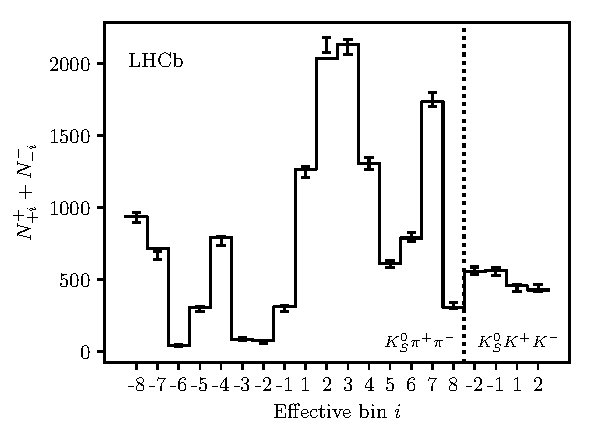
\includegraphics[width=0.48\columnwidth]{figures/analysis/cpfit_cross_check_plots/paper_yields_dk.pdf}
    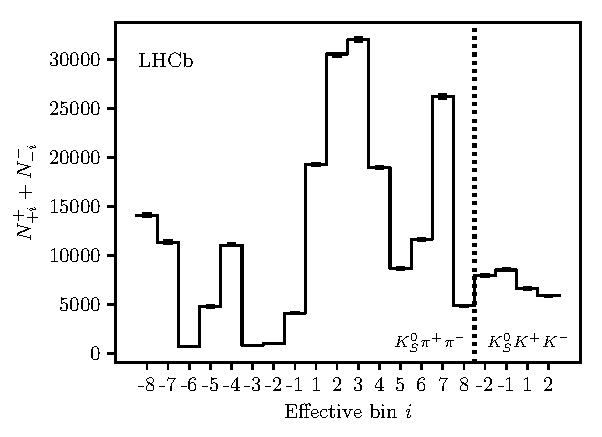
\includegraphics[width=0.48\columnwidth]{figures/analysis/cpfit_cross_check_plots/paper_yields_dpi.pdf}
    \caption{Comparison of (lines) the predicted yield given the determined \CP observables and (error bars) the yield obtained in fits to data where each yield is an independent parameter. The yields are shown for (left) \BtoDK decays and (right) \BtoDpi decays. The LL and DD categories have been combined, as has the \Bp and \Bm yields for each effective Dalitz bin, defined as bin $+i$ for \Bp decays and bin $-i$ for \Bm decays.}
    \label{fig:yield_cross_check}
\end{figure}

\begin{figure}[tb]
    \centering
    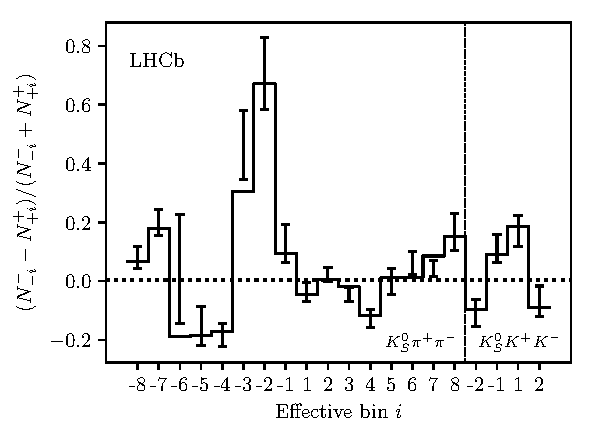
\includegraphics[width=0.48\columnwidth]{figures/analysis/cpfit_cross_check_plots/paper_asym_dk.pdf}
    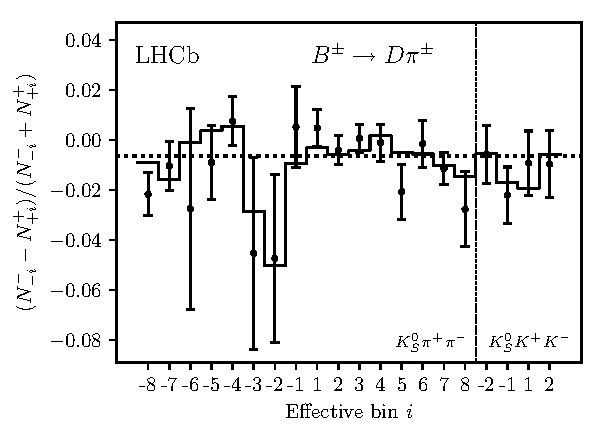
\includegraphics[width=0.48\columnwidth]{figures/analysis/cpfit_cross_check_plots/paper_asym_dpi.pdf}
    \caption{The bin-by-bin asymmetries $(N^-_{-i}-N^+_{+i})/(N^-_{-i}+N^+_{+i})$ for each Dalitz-plot bin number for (left) \BtoDK decays and (right) \BtoDpi decays. The prediction from the central values of the \CP-violation observables is shown with a solid line and the asymmetries obtained in fits with independent bin yields are shown with the error bars. The predicted asymmetries in a fit that does not allow for \CP violation are shown with a dotted line.}
    \label{fig:asym_cross_check}
\end{figure}

% subsubsection compare_results_obtained_with_different_binning_schemes (end)

% subsection cross_checks (end)
% section fit_of_cp_observables (end)


\subsubsection{Fitting subsets of the data separately} % (fold)
\label{ssub:fitting_subsets_of_the_data_separately}

One cross check is carrying out, by determining the \CP observables using a number of independent sub samples of the data set separately.  This is done for the following following data splits

\begin{itemize}
    \item Fig.~\ref{fig:subsample_result_comparisons_track} shows the same plots, comparing the fits to the data set split by \KS track type.
    \item Fig.~\ref{fig:subsample_result_comparisons_d_decay} shows the same plots, comparing the fits to the data set split by whether the \D meson decays to the \Kspipi or \KsKK final state.

    \item Fig.~\ref{fig:subsample_result_comparisons_year} shows the two dimensional log likelihood contours for the observables for fits to the Run~1, 2015+16, 2017 and 2018 datasets separately 
    \item Fig.~\ref{fig:subsample_result_comparisons_trigger} shows the same plots, comparing the fits to the data set split by whether the candidate event was triggered by one of the signal particles at the hardware level (TOS), or by another particle in the underlying event (TIS).
    \item Fig.~\ref{fig:subsample_result_comparisons_polarity} shows the same plots, comparing the fits to the data set split the magnet polarity during data taking.
\end{itemize}
All figures show the Gaussian likelihood contours corresponding to the statistical uncertainties. There is good agreement between the results in all cases, given that in each cases the sub datasets are independent and therefore the statistical errors are uncorrelated.  

\begin{figure}[tp]
    \centering

\begin{subfigure}{0.95\columnwidth}
    \centering
    \hspace*{-1.5cm}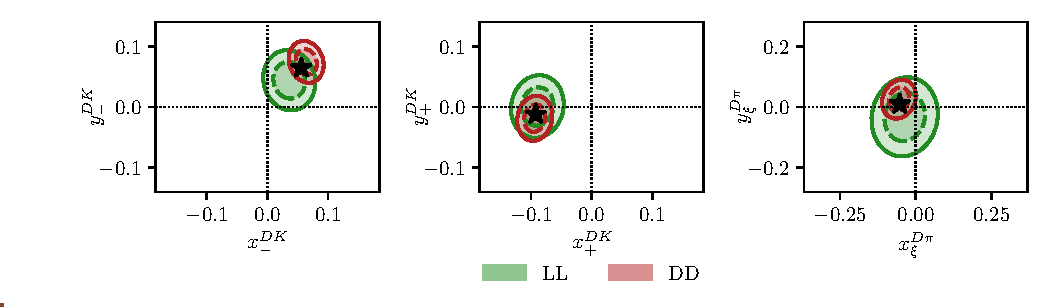
\includegraphics[width=\textwidth]{figures/analysis/cpfit_cross_check_plots/compare_tracks.pdf}\vspace{-2.5mm}

    \caption{\label{fig:subsample_result_comparisons_track}}
\end{subfigure}
\begin{subfigure}{0.95\columnwidth}
    \centering
    \hspace*{-1.5cm}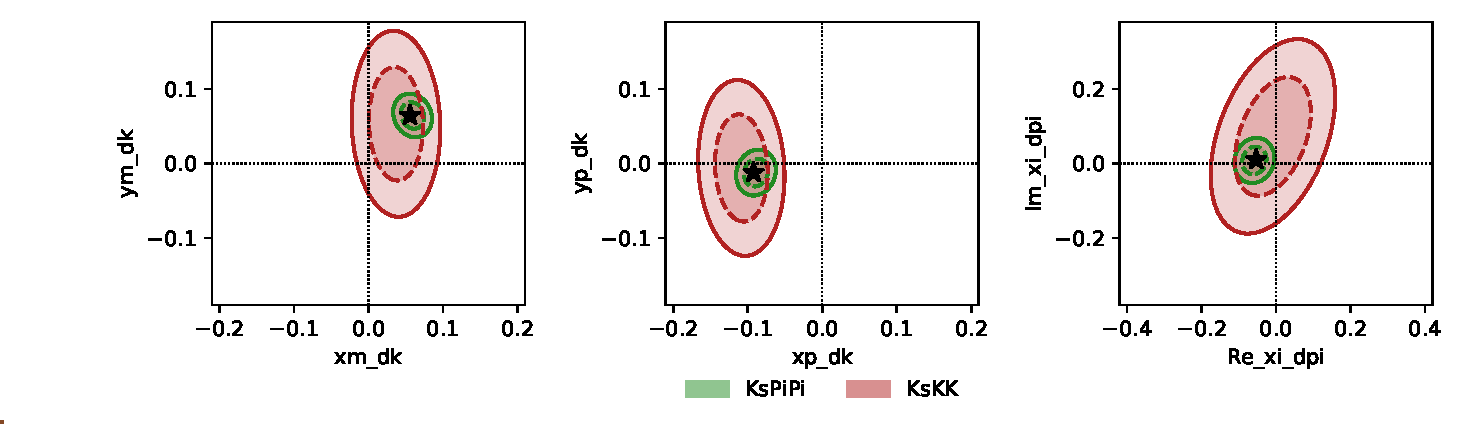
\includegraphics[width=\textwidth]{figures/analysis/cpfit_cross_check_plots/compare_d_decay.pdf}\vspace{-2.5mm}

    \caption{\label{fig:subsample_result_comparisons_d_decay}}
\end{subfigure}
    \caption{Comparison of the 68\,\% and 95\,\% confidence regions for (left) $(\xmdk, \ymdk)$, (centre) $(\xpdk, \ypdk)$, and (right) $(\xxidpi, \yxidpi)$ obtained from fits to sub sets of the data set. The uncertainties are statistical only. The central values of the default fit are shown with a black star. The dataset is split by (a)  LL and DD \KS types and (b) \D decay mode.}
    \label{fig:subsample_result_comparisons}
\end{figure}


\begin{figure}[tp]
    \centering
\begin{subfigure}{0.95\columnwidth}
    \centering
    \hspace*{-1.5cm}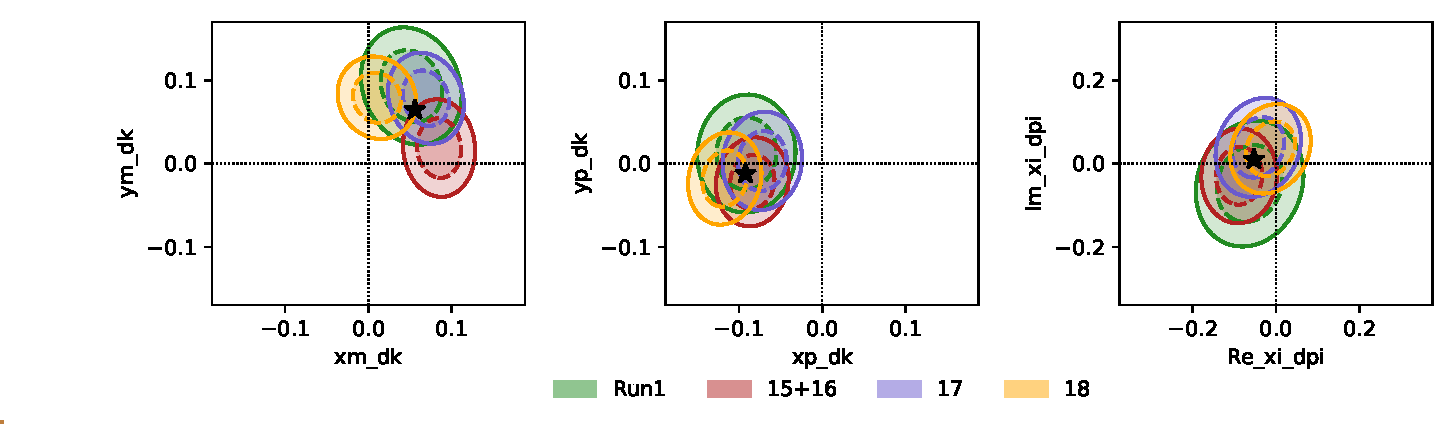
\includegraphics[width=\textwidth]{figures/analysis/cpfit_cross_check_plots/compare_years.pdf}\vspace{-2.5mm}

    \caption{\label{fig:subsample_result_comparisons_year}}
\end{subfigure}

\begin{subfigure}{0.95\columnwidth}
    \centering
    \hspace*{-1.5cm}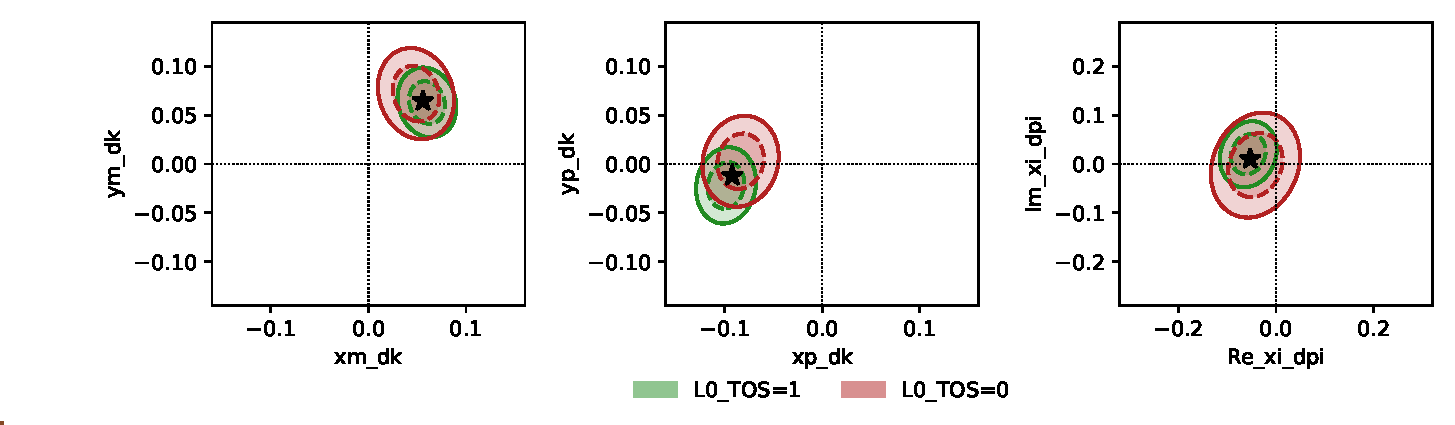
\includegraphics[width=\textwidth]{figures/analysis/cpfit_cross_check_plots/compare_TOS.pdf}\vspace{-2.5mm}

    \caption{\label{fig:subsample_result_comparisons_trigger}}
\end{subfigure}
\begin{subfigure}{0.95\columnwidth}
    \centering
    \hspace*{-1.5cm}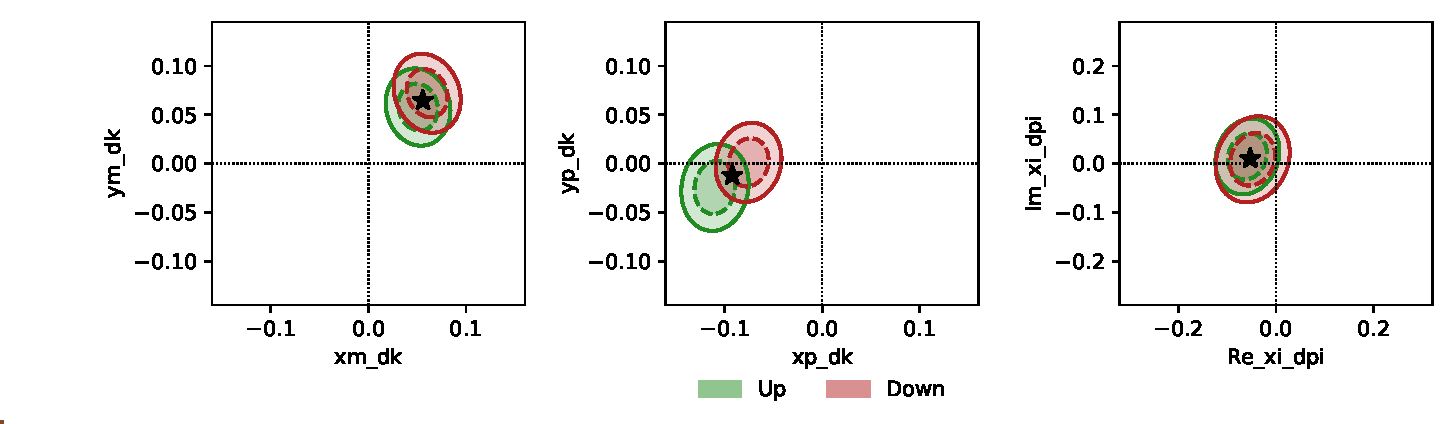
\includegraphics[width=\textwidth]{figures/analysis/cpfit_cross_check_plots/compare_mags.pdf}\vspace{-2.5mm}

    \caption{\label{fig:subsample_result_comparisons_polarity}}
\end{subfigure}

    \caption{Comparison of the 68\,\% and 95\,\% confidence regions for (left) $(\xmdk, \ymdk)$, (centre) $(\xpdk, \ypdk)$, and (right) $(\xxidpi, \yxidpi)$ obtained from fits to sub sets of the data set. The uncertainties are statistical only. The central values of the default fit are shown with a black star. The dataset is split by (a) data taking year, (b) trigger category, and (c) magnet polarity.}
    \label{fig:subsample_result_comparisons_2}
\end{figure}
% subsubsection fitting_subsets_of_the_data_separately (end)

% \subsubsection{Examining constraints from a subset of the bins independently} % (fold)
% \label{ssub:examining_constraints_from_a_subset_of_the_bins_independently}

% subsection compare_results_obtained_with_different_strong_phase_inputs (end)

\subsubsection{Constraints from a subset of bins} % (fold)
\label{ssub:constraints_from_a_subset_of_bins}

\begin{figure}[tbp]
    \centering
    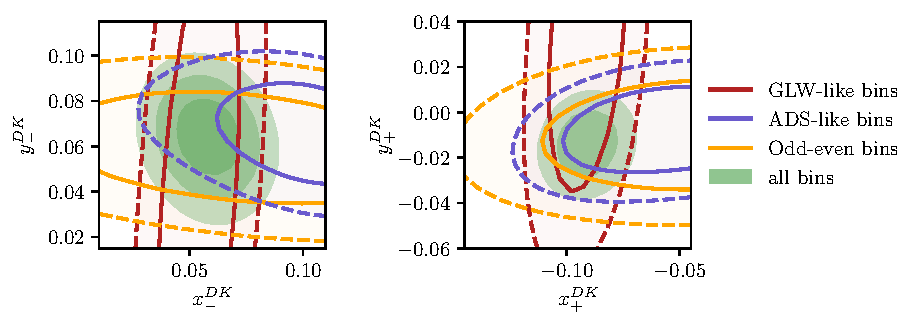
\includegraphics[width=0.95\columnwidth]{figures/analysis/cpfit_cross_check_plots/bin_by_bin_constraints.pdf}
    \caption{Constraints on the \BtoDK observables from the signal yields of different subsets the \DtoKspp Dalitz bins, using the bin categorisation developed in Section~\ref{sub:relation_to_glw_and_ads_measurements}.}
    \label{fig:bin_by_bin_likelihoods}
\end{figure}

An alternative way to subdivide the data is to examine the constraints from a subset of bins individually; this forms as a cross check because the observables favoured by each sub set should be compatible, and also serves as a useful illustration of the features of the BPGGSZ method. Likelihood contours for $(\xpmdk, \ypmdk)$ are shown in Fig.~\ref{fig:bin_by_bin_likelihoods}, obtained using the binned yields in the \DtoKspp bins, determined in the fits of individual bin yields described in Section~\ref{ssub:_directly_fitting_the_signal_yields}. The bins are split by whether they are ADS-like, GLW-like, or Odd-even according to the classification in Section~\ref{sub:relation_to_glw_and_ads_measurements}. It is clear that the likelihood regions show a reasonable overlap, and also how it is the GLW bins that constrain the $x_\pm$ parameter, while the Odd-even and ADS-like bins provide the ability to constrain the $y_\pm$ parameters.

% subsubsection constraints_from_a_subset_of_bins (end)

\subsubsection{\texorpdfstring{Significantly reducing the \BtoDpi to \BtoDK cross feed}{Significantly reducing the BtoDpi to BtoDK cross feed}} % (fold)
\label{ssub:significantly_tightening_the_bachelor_pid_cut}

One of the dominant backgrounds in the signal region of the \BtoDK channel is from partly reconstructed $\B\to\D\pi X$ decays where the bachelor pion is misidentified as a kaon. The background mode is well described by the included shape component, and included in all relevant systematic studies. Nevertheless, an additional cross check is carried out to ensure that it is not having a significant effect on the fit: the analysis is repeated with PID requirement of $\texttt{PIDK}>12$ required to place a candidate in the \BtoDK category, instead of $\texttt{PIDK}>4$. With this requirement 99.7\,\% of \BtoDpi decays are correctly identified, making the cross-feed component in the \BtoDK channels significantly smaller than in the default fit. This is clearly visible in Fig.~\ref{fig:pid12_fits}, where the fit projections for the global fit of the \DtoKspipi modes are shown. In return, the probability of correctly identifying a kaon companion drops to about 68--69\,\%, resulting in a smaller effective signal yield. 

The measurement results are compared in Table~\ref{tab:pid12}, where the differences in central value are seen to be reasonably small. It is not trivial to determine whether the difference is statistically significant or not: the same candidates are analysed in both cases, the difference being that a number of candidates that are placed in the \BtoDK category in the nominal fit are placed in the \BtoDpi category in the alternative fit. The uncertainty will not be 100\,\% correlated because signal events that move from the $\D K$ to $\D\pi$  category are placed in a region with high background; however, this is somewhat compensated for by candidates that remain in the $\D K$  category gaining  statistical power due to the increased purity. An estimate of the expected statistical fluctuation can be determined by taking the difference of the statistical uncertainties in quadrature. Using this estimate, the observed shifts are found to consistent with statistical fluctuation, and thus there is no sign of the background from $\Dpi\to\DK$ cross-feed causing issues. 


\begin{figure}[tbp]
    \centering
    \includegraphics[width=0.98\columnwidth]{figures/analysis/pretty_fit_tightPID_d2kspp_LL.pdf}
    \includegraphics[width=0.98\columnwidth]{figures/analysis/pretty_fit_tightPID_d2kspp_DD.pdf}
    \caption{Fit projections for fits to the \DtoKspipi candidates with a companion \texttt{PIDK} requirement at 12 instead of 4 used to split into (left) \BtoDK and (right) \BtoDpi candidates, for the (top)  LL and (bottom) DD categories.}
    \label{fig:pid12_fits}
\end{figure}

\begin{table}[tbp]
\centering
\caption{Results of running the measurement with the default \texttt{PIDK} requirement at 4 used to separate \BtoDK and \BtoDpi candidates, as well as with an alternative \texttt{PIDK} requirement at 12, resulting in much lower cross-feed from misidentified \BtoDpi decays. We also show the pulls, defined as $\Delta x / \sqrt{|\sigma^2_{PIDK>12} - \sigma^2_{PIDK>4}|}$ as described in the main text body. The comparison was made before the BESIII measurement of the \DtoKsKK strong-phase inputs became available; therefore the fits use the CLEO-only results~\cite{CLEOCISI} for this mode, which explains why the results quoted for $\texttt{PIDK}>4$ differ slightly from the nominal fit results.
\label{tab:pid12}}
    

\begin{tabular}{c|cccc}
\toprule
    Parameter & $\texttt{PIDK}>4$ & $\texttt{PIDK}>12$ & $\sigma=\sqrt{\sigma^2_{PIDK>12} - \sigma^2_{PIDK>4}}$ & Pull \\
    \midrule
    \xmdk   & $\phantom{-} 5.59 \pm  0.96$& $\phantom{-} 5.82 \pm  1.01$& $ 0.30 $& $ 0.77 $ \\
    \ymdk   & $\phantom{-} 6.45 \pm  1.14$& $\phantom{-} 6.86 \pm  1.19$& $ 0.36 $& $ 1.13 $ \\
    \xpdk   & $           -9.21 \pm  0.96$& $           -8.94 \pm  1.01$& $ 0.30 $& $ 0.93 $ \\
    \ypdk   & $           -1.21 \pm  1.20$& $           -0.94 \pm  1.26$& $ 0.37 $& $ 0.71 $ \\
    \xxidpi & $           -5.30 \pm  1.99$& $           -5.13 \pm  2.02$& $ 0.32 $& $ 0.52 $ \\
    \yxidpi & $\phantom{-} 1.03 \pm  2.34$& $\phantom{-} 1.71 \pm  2.33$& $ 0.28 $& $ 2.40 $ \\
    \bottomrule
\end{tabular}

\end{table}

\subsubsection{Compare results obtained with different strong-phase inputs} % (fold)
\label{ssub:compare_results_obtained_with_different_strong_phase_inputs}
{}
It is interesting to compare the results obtained with different strong-phase inputs. This is done in Fig.~\ref{fig:compare_cisi_results}, where the default fit results are compared to those obtained if the \CP fit is done with the CLEO-only inputs~\cite{CLEOCISI}, and with the model predictions from the 2018~Belle~model~\cite{Belle2018} and the 2008~BaBar~model~\cite{BABAR2008}. For the measurements, only the strong-phase-related uncertainties are included in the plot, since the statistical uncertainties are correlated. All results are found to agree well.

\begin{figure}[tbp]
    \centering
    \includegraphics[width=\columnwidth]{figures/analysis/systematics/strong_phase_inputs.pdf}
    \caption{Fit results for (left) $(\xmdk, \ymdk)$, (centre) $(\xpdk, \ypdk)$, and (right) $(\xxidpi, \yxidpi)$ depending on strong-phase inputs, shown relative to the default fit results. The included results are based on (green) the BESIII-CLEO combination, which is the default, (red) the CLEO-only results, (blue dot) the 2018~Belle~model~\cite{Belle2018} and (orange dot) the 2008~BaBar~model~\cite{BABAR2008}. For the measurements, only strong-phase related uncertainties are included in the plotted confidence regions.}
    \label{fig:compare_cisi_results}
\end{figure}

% \subsubsection{Repeat analysis with stricter selection requirements} % (fold)
% \label{ssub:repeat_analysis_with_stricter_selection_requirements}

% It is investigated whether the obtained results depend on a range of different parameters used in the selection. For each parameter, four intervals are chosen that split the final data set into four subsamples of approximately equal size, and the two-stage fit is repeated for each subsample in isolation. The results are compared to the default result for the BDT variable, the charmless cut variable $\Delta z^{BD}_{\text{significance}}$, and the \KS flight-distance $\chi^2$ in Fig.~\ref{fig:cut_val_scans_1}, and for the DTF $\chi^2/$NDOF, the \KS mass, and the \D mass in Fig.~\ref{fig:cut_val_scans_2}. In each case, we calculate the $\chi^2$ of the four measurements with respect to the default value, and calculate a corresponding $p$-value for a $\chi^2$-distribution with three degrees of freedom (since we compare to the average of the four independent measurements). We see no statistically significant trends.
% % subsubsection repeat_analysis_with_stricter_selection_requirements (end)


% \begin{figure}[tp]
%     \centering
%     % \begin{subfigure}{\columnwidth}
%     %         \includegraphics[width=\columnwidth]{figs/cp_fit/cross_check_plots/scan_MVA_cut.pdf}
%     %         \caption{}
%     % \end{subfigure}
%     % \begin{subfigure}{\columnwidth}
%     % \includegraphics[width=\columnwidth]{figs/cp_fit/cross_check_plots/scan_BD_ZSIG_cut.pdf}
%     %         \caption{}
%     % \end{subfigure}
%     % \begin{subfigure}{\columnwidth}
%     % \includegraphics[width=\columnwidth]{figs/cp_fit/cross_check_plots/scan_Ks_FDCHI2_ORIVX_cut.pdf}
%     %         \caption{}
%     % \end{subfigure}
%     \caption{(Error bars) Results obtained for each of the observables, when the fit is repeated splitting the final data set into four independent subsets, depending on the value of (a) the BDT variable (denoted \texttt{MVA}), (b) the charmless cut variable $\Delta z^{BD}_{\text{significance}}$ (\texttt{BD\_ZSIG}), and (c) the \KS flight-distance $\chi^2$ (\texttt{Ks\_FDCHI2\_ORIVX}). In each case, we calculate the $\chi^2$ of the four measurements with respect to the default value (grey band), and calculate a corresponding $p$-value for a $\chi^2$-distribution with three degrees of freedom.}
%     \label{fig:cut_val_scans_1}
% \end{figure}

% \begin{figure}[tp]
%     \centering
%     % \begin{subfigure}{\columnwidth}
%     % \includegraphics[width=\columnwidth]{figs/cp_fit/cross_check_plots/scan_Bu_constD0KSPV_CHI2NDOF_cut.pdf}
%     %         \caption{}
%     % \end{subfigure}
%     % \begin{subfigure}{\columnwidth}
%     % \includegraphics[width=\columnwidth]{figs/cp_fit/cross_check_plots/scan_Bu_constKSPV_D0_M_cut.pdf}
%     %         \caption{}
%     % \end{subfigure}
%     % \begin{subfigure}{\columnwidth}
%     % \includegraphics[width=\columnwidth]{figs/cp_fit/cross_check_plots/scan_Bu_constD0PV_KS0_M_cut.pdf}
%     %         \caption{}
%     % \end{subfigure}
%     \caption{(Error bars) Results obtained for each of the observables, when the fit is repeated splitting the final data set into four independent subsets, depending on the value of (a) the DTF $\chi^2/$NDOF (denoted \texttt{Bu\_constD0KSPV\_CHI2NDOF}), (b) the \KS mass (\texttt{Bu\_constD0PV\_KS0\_M})), and (c) the \D mass (\texttt{Bu\_constKSPV\_D0\_M}). In each case, we calculate the $\chi^2$ of the four measurements with respect to the default value (grey band), and calculate a corresponding $p$-value for a $\chi^2$-distribution with three degrees of freedom.}
%     \label{fig:cut_val_scans_2}
% \end{figure}


% subsection cross_checks (end)

% section measurement_of_the_cp_violation_observables (end)
